% IndusOPT paper -- arXiv preprint (single column).
% Build: latexmk -pdf main.tex   (or: tectonic main.tex)
% Numbers are injected from the macro block below, originally generated by
% gen_numbers.py. Regenerate that block after any dataset change instead of
% editing figures in the text.
\documentclass[11pt]{article}

\usepackage[margin=1in]{geometry}
\usepackage[T1]{fontenc}
\usepackage[utf8]{inputenc}
% amsmath/amssymb must precede newtx: newtxmath redefines \Bbbk and friends,
% and loading it first makes amssymb abort with "Command \Bbbk already defined".
\usepackage{amsmath,amssymb}
\IfFileExists{newtxtext.sty}{\usepackage{newtxtext,newtxmath}}{\usepackage{lmodern}}
\usepackage{microtype}
\usepackage{booktabs}
\usepackage{multirow}
\usepackage{graphicx}
\usepackage{xspace}
\usepackage{caption}
\usepackage{capt-of}
\usepackage{subcaption}
\usepackage[numbers,sort&compress]{natbib}
\usepackage{xcolor}
\usepackage[colorlinks=true,linkcolor=blue!60!black,citecolor=blue!60!black,urlcolor=blue!60!black]{hyperref}
\usepackage{enumitem}
\setlist{topsep=2pt,itemsep=1pt}
\usepackage{tikz}
\usetikzlibrary{positioning,arrows.meta,calc}
% Figure palette (matches make_paper_figures.py).
\definecolor{figblue}{HTML}{2A78D6}
\definecolor{figorange}{HTML}{EB6834}
\definecolor{figaqua}{HTML}{1BAF7A}
\definecolor{figink}{HTML}{52514E}
\definecolor{figbluebg}{HTML}{EDF4FC}
\definecolor{figorangebg}{HTML}{FDEFE8}

\usepackage[most]{tcolorbox}
% Before/after comparison boxes for the defect case studies (Section 4).
\definecolor{badbg}{HTML}{FDF1EA}
\definecolor{badln}{HTML}{B8501F}
\definecolor{goodbg}{HTML}{ECF3FC}
\definecolor{goodln}{HTML}{1D5FAE}
\newtcolorbox{badbox}[1][Before: as submitted]{colback=badbg,colframe=badln,
  boxrule=0.4pt,arc=1.5pt,left=4pt,right=4pt,top=3pt,bottom=3pt,
  fonttitle=\bfseries\scriptsize,coltitle=white,title=#1}
\newtcolorbox{goodbox}[1][After: as repaired]{colback=goodbg,colframe=goodln,
  boxrule=0.4pt,arc=1.5pt,left=4pt,right=4pt,top=3pt,bottom=3pt,
  fonttitle=\bfseries\scriptsize,coltitle=white,title=#1}
% Two boxes side by side, where #1 is the left body and #2 the right body.
\newcommand{\baside}[2]{%
  \noindent\begin{minipage}[t]{0.485\linewidth}\begin{badbox}#1\end{badbox}\end{minipage}%
  \hfill%
  \begin{minipage}[t]{0.485\linewidth}\begin{goodbox}#2\end{goodbox}\end{minipage}}
\newcommand{\bacode}[1]{{\ttfamily\scriptsize\setlength{\baselineskip}{8.4pt}#1}}
\newcommand{\batext}[1]{{\footnotesize #1}}

% ===========================================================================
% Numbers (was numbers.tex).
% Auto-generated by paper/gen_numbers.py -- do not edit by hand.
% ===========================================================================
% Dataset statistics: computed from domains/*/meta.yaml at generation time.
\newcommand{\NumProblems}{17\xspace}
\newcommand{\NumInstances}{128\xspace}
\newcommand{\NumSubdomains}{15\xspace}
\newcommand{\NumOwners}{9\xspace}
\newcommand{\MinScale}{33\xspace}
\newcommand{\MaxScale}{5,310,086\xspace}
\newcommand{\BandSmall}{3\xspace}
\newcommand{\BandMedium}{95\xspace}
\newcommand{\BandLarge}{22\xspace}
\newcommand{\BandVeryLarge}{8\xspace}
\newcommand{\NumMILP}{12\xspace}
\newcommand{\NumIP}{2\xspace}
\newcommand{\NumLP}{1\xspace}
\newcommand{\NumQP}{1\xspace}
\newcommand{\NumMINLP}{1\xspace}
\newcommand{\NumPublic}{15\xspace}
\newcommand{\NumInternal}{2\xspace}
\newcommand{\NumOriginReal}{2\xspace}
\newcommand{\NumOriginHybrid}{2\xspace}
\newcommand{\NumOriginSynthetic}{13\xspace}
\newcommand{\MinAxes}{2\xspace}
\newcommand{\MaxAxes}{7\xspace}
\newcommand{\DatasetCommit}{\texttt{4d851173f8-dirty}\xspace}
% Defect ledger, from paper/defect_ledger.json.
\newcommand{\NumPullRequests}{101\xspace}
\newcommand{\NumMergedPRs}{92\xspace}
\newcommand{\NumDefectClasses}{13\xspace}
\newcommand{\NumDefects}{40\xspace}
\newcommand{\NumDefectsMechanical}{23\xspace}
% Drop-one coverage, from paper/coverage_results.json.
\newcommand{\NumAudited}{12\xspace}
\newcommand{\NumNotAudited}{5\xspace}
\newcommand{\NumFamiliesAudited}{51\xspace}
\newcommand{\NumBlindSpots}{1\xspace}
\newcommand{\NumWeakFamilies}{4\xspace}
% Repeated runs and the language pilot, from paper/repeats.json.
\newcommand{\RepeatProblems}{12\xspace}
\newcommand{\RepeatRuns}{3\xspace}
\newcommand{\RepeatUnstable}{3\xspace}
\newcommand{\RepeatStable}{9\xspace}
\newcommand{\LangPairs}{3\xspace}
% Optimality audit, from paper/audit_results.json.
\newcommand{\AuditConsistent}{109\xspace}
\newcommand{\AuditUnproven}{15\xspace}
\newcommand{\AuditContradicted}{0\xspace}
\newcommand{\AuditSkipped}{4\xspace}
% Structural characterisation, from paper/structure.json.
\newcommand{\MinFamilies}{2\xspace}
\newcommand{\MaxFamilies}{18\xspace}
\newcommand{\MedFamilies}{4\xspace}
\newcommand{\NumPureInteger}{8\xspace}
\newcommand{\NumContinuous}{2\xspace}

% Evaluation headline numbers: recomputed from the archived per-run
% result.json of the reported sweep (scheme 82755f3a0583), with the
% offline cross-check correction of 判据复判-20260821-128实例 applied.
% These reproduce the published post-rejudge table exactly.
\newcommand{\NumJudgeable}{113\xspace}
\newcommand{\NumUnjudgeable}{15\xspace}
\newcommand{\NumRuns}{68\xspace}
\newcommand{\NumInstanceRuns}{512\xspace}
\newcommand{\ComposerWithAnn}{84/113\xspace}
\newcommand{\ComposerNoAnn}{85/113\xspace}
\newcommand{\OpusWithAnn}{96/113\xspace}
\newcommand{\OpusNoAnn}{93/113\xspace}
\newcommand{\ComposerWithAnnPct}{74.3\%\xspace}
\newcommand{\ComposerNoAnnPct}{75.2\%\xspace}
\newcommand{\OpusWithAnnPct}{85.0\%\xspace}
\newcommand{\OpusNoAnnPct}{82.3\%\xspace}
% Conservative denominator: all instances, unjudgeable counted as not passed.
\newcommand{\ComposerWithAnnAllPct}{65.6\%\xspace}
\newcommand{\ComposerNoAnnAllPct}{66.4\%\xspace}
\newcommand{\OpusWithAnnAllPct}{75.0\%\xspace}
\newcommand{\OpusNoAnnAllPct}{72.7\%\xspace}
% Strict tier: passes on which the bidirectional cross-check actively
% confirmed feasibility in the reference model, rather than abstaining.
\newcommand{\StrictComposerWithAnn}{15/113\xspace}
\newcommand{\StrictComposerNoAnn}{6/113\xspace}
\newcommand{\StrictOpusWithAnn}{14/113\xspace}
\newcommand{\StrictOpusNoAnn}{6/113\xspace}
\newcommand{\StrictComposerWithAnnPct}{13.3\%\xspace}
\newcommand{\StrictComposerNoAnnPct}{5.3\%\xspace}
\newcommand{\StrictOpusWithAnnPct}{12.4\%\xspace}
\newcommand{\StrictOpusNoAnnPct}{5.3\%\xspace}
\newcommand{\CrossConfirmed}{42\xspace}
\newcommand{\CrossAbstained}{401\xspace}
\newcommand{\CrossViolated}{0\xspace}
\newcommand{\CrossNotRun}{69\xspace}
\newcommand{\StrictProblems}{3\xspace}
% Rejudge: 36 false 'infeasible-in-reference' alarms, 30 flipped verdicts.
\newcommand{\RejudgeFalseAlarms}{36\xspace}
\newcommand{\RejudgeFlipped}{30\xspace}

% MIPLIB-NL comparator numbers, read off the published tables of
% arXiv:2602.10450 (ICML 2026) rather than paraphrased. Table 1 is Pass@1,
% Table 8 Pass@8, and Table 9 the execution-level failure rate, with the
% MIPLIB-NL column last in each. The 17.9% figure widely quoted from that
% paper is Table 1's Avg row over ALL evaluated systems, that is, bare LLMs,
% fine-tuned specialists and NL-to-Opt pipelines together, rather than the
% bare-LLM average.
% The nine bare LLMs it evaluates average 26.9% (DeepSeek-V3.2 23.81 /
% -Think 22.38, Qwen3-Max 21.43 / -Thinking 21.43, Claude-Sonnet-4.5 24.23 /
% -Thinking 30.00, Gemini-3-Pro 36.19, GPT-5.1 39.05, GPT-5.1-CodeX 23.33).
% Specialists at Pass@1: OptMATH-7B 0.00, SIRL-7B 0.48, ORLM-8B 0.58,
% SIRL-32B 1.43, OptMATH-32B 5.50.
\newcommand{\MiplibInstances}{223\xspace}
\newcommand{\MiplibAllAvg}{17.9\%\xspace}
\newcommand{\MiplibBareAvg}{26.9\%\xspace}
\newcommand{\MiplibBareLo}{21.4\%\xspace}
\newcommand{\MiplibBareBest}{39.1\%\xspace}
\newcommand{\MiplibSpecialistHi}{5.5\%\xspace}
\newcommand{\MiplibPassEight}{21.9\%\xspace}
\newcommand{\MiplibExecFail}{47.6\%\xspace}
% Solve regime (scheme fingerprint 82755f3a0583 -> 001ef9239e01 after fix).
\newcommand{\SolverTimeLimit}{900\xspace}
\newcommand{\ScoreTol}{$10^{-6}$\xspace}
% Inline-prompt budget (paper/measure_inline_budget.py).
\newcommand{\InlineMedianKB}{13.5\xspace}
\newcommand{\InlineMaxMB}{23\xspace}
\newcommand{\InlineOverSmall}{21\xspace}
\newcommand{\InlineOverSmallPct}{16\%\xspace}
\newcommand{\InlineOverLarge}{11\xspace}
\newcommand{\InlineOverLargePct}{9\%\xspace}

% ===========================================================================
% Problem table rows (was problems_table.tex).
% Auto-generated by paper/gen_numbers.py -- do not edit by hand.
% ===========================================================================
\newcommand{\ProblemRows}{%
\texttt{CBG-Camera-JPEGQuantizationTable} & MILP & 8 & 1,471 & 2,457 & 3 & 1.00 \\
\texttt{CBG-Camera-VideoStabilization-L1} & LP & 8 & 520 & 1,204 & 4 & 0.00 \\
\texttt{CBG-Camera-VideoStabilization-L2} & QP & 8 & 160 & 358 & 2 & 0.00 \\
\texttt{CBG-Communication-RailCellHandover} & MILP & 5 & 34 & 620 & 6 & 0.62 \\
\texttt{CBG-HarmonyOS-CriticalThreadOpt} & MILP & 5 & 1,046 & 1,386 & 3 & 1.00 \\
\texttt{CBG-HarmonyOS-MemoryEviction} & MILP & 8 & 161 & 654 & 4 & 1.00 \\
\texttt{Compute-CAE-SparseLA-LDLSymmetricPivoting} & IP & 6 & 264 & 4,054 & 2 & 1.00 \\
\texttt{Compute-CAE-SparseLA-LUPivotReordering} & IP & 6 & 415 & 5,994 & 2 & 1.00 \\
\texttt{Compute-Cluster-CrossPodLoadBalancing} & MILP & 10 & 301 & 34,145 & 3 & 0.17 \\
\texttt{Compute-LLM-MoEExpertLoadBalance} & MINLP & 5 & 204 & 761,018 & 5 & 0.52 \\
\texttt{Compute-TBE-MemoryAllocation} & MILP & 8 & 3,141 & 176,099 & 18 & 1.00 \\
\texttt{Energy-Microgrid-SizingAndOperation} & MILP & 10 & 6,012 & 5,310,086 & 13 & 0.29 \\
\texttt{Energy-VPP-DayAheadAdjustableLoadScheduling} & MILP & 15 & 5,356 & 1,269,056 & 17 & 0.19 \\
\texttt{ICT-DataCom-LoadBalancing-SingleAndMultitimestamp} & MILP & 8 & 33 & 677 & 3 & 0.23 \\
\texttt{ICT-DataCom-NetworkPlanning-CapacityExpansion} & MILP & 8 & 528 & 7,336 & 4 & 0.31 \\
\texttt{ICT-OpticalNetwork-NetworkPlanning-LinkProtection} & MILP & 5 & 974 & 14,424 & 10 & 1.00 \\
\texttt{ICT-OpticalNetwork-NetworkPlanning-PathProtection} & MILP & 5 & 198 & 5,172 & 8 & 1.00 \\}

% ===========================================================================
% Coverage table rows (was coverage_table.tex).
% Auto-generated by paper/gen_numbers.py from coverage_results.json.
% ===========================================================================
\newcommand{\CoverageRows}{%
{\ttfamily CBG-\allowbreak Camera-\allowbreak JPEGQuantization\allowbreak Table} & C1~6/8, C2~8/8, C3~5/8 \\
{\ttfamily CBG-\allowbreak Camera-\allowbreak Video\allowbreak Stabilization-\allowbreak L1} & C1~2/8, C2~7/8, C3~8/8, C4~8/8 \\
{\ttfamily CBG-\allowbreak Camera-\allowbreak Video\allowbreak Stabilization-\allowbreak L2} & C1~2/8, C2~7/8 \\
{\ttfamily CBG-\allowbreak Communication-\allowbreak Rail\allowbreak Cell\allowbreak Handover} & C1~5/5, C2~5/5, C3~3/5, C4~3/5, C5~3/5, C6~5/5 \\
{\ttfamily CBG-\allowbreak Harmony\allowbreak OS-\allowbreak Critical\allowbreak Thread\allowbreak Opt} & C1~5/5, \textbf{C2~0/5}, C3~5/5 \\
{\ttfamily CBG-\allowbreak Harmony\allowbreak OS-\allowbreak Memory\allowbreak Eviction} & C1~7/8, C2~4/8, C3~8/8, C4~8/8 \\
{\ttfamily Compute-\allowbreak CAE-\allowbreak Sparse\allowbreak LA-\allowbreak LDLSymmetric\allowbreak Pivoting} & C1~6/6, C2~1/6 \\
{\ttfamily Compute-\allowbreak CAE-\allowbreak Sparse\allowbreak LA-\allowbreak LUPivot\allowbreak Reordering} & C1~6/6, C2~5/6 \\
{\ttfamily ICT-\allowbreak Data\allowbreak Com-\allowbreak Load\allowbreak Balancing-\allowbreak Single\allowbreak And\allowbreak Multitimestamp} & C1~8/8, C2~8/8, C3~8/8 \\
{\ttfamily ICT-\allowbreak Data\allowbreak Com-\allowbreak Network\allowbreak Planning-\allowbreak Capacity\allowbreak Expansion} & C1~8/8, C2~8/8, C3~8/8, C4~8/8 \\
{\ttfamily ICT-\allowbreak Optical\allowbreak Network-\allowbreak Network\allowbreak Planning-\allowbreak Link\allowbreak Protection} & C1~5/5, C2~5/5, C3~1/5, C4~5/5, C5~5/5, C6~5/5, C7~5/5, C8~4/5, C9~5/5, C10~5/5 \\
{\ttfamily ICT-\allowbreak Optical\allowbreak Network-\allowbreak Network\allowbreak Planning-\allowbreak Path\allowbreak Protection} & C1~5/5, C2~5/5, C3~5/5, C4~5/5, C5~4/5, C6~5/5, C7~5/5, C8~5/5 \\
{\ttfamily Compute-\allowbreak Cluster-\allowbreak Cross\allowbreak Pod\allowbreak Load\allowbreak Balancing} & \emph{not audited, because drop-one needs one re-solve per family per instance, and a single instance takes up to 31 min} \\
{\ttfamily Compute-\allowbreak LLM-\allowbreak Mo\allowbreak EExpert\allowbreak Load\allowbreak Balance} & \emph{not audited, because this is an MINLP whose baseline solve alone does not finish reliably within budget} \\
{\ttfamily Compute-\allowbreak TBE-\allowbreak Memory\allowbreak Allocation} & \emph{not audited, being of the same order as Cross-pod, with the largest instances reaching 1.8e5 vars+cons} \\
{\ttfamily Energy-\allowbreak Microgrid-\allowbreak Sizing\allowbreak And\allowbreak Operation} & \emph{not audited, because the largest instance is 5.3e6 vars+cons and exhausts memory on a single solve} \\
{\ttfamily Energy-\allowbreak VPP-\allowbreak Day\allowbreak Ahead\allowbreak Adjustable\allowbreak Load\allowbreak Scheduling} & \emph{not audited, because 17 families x 15 instances of re-solves take hours of wall clock} \\}

% ===========================================================================
% Defect table rows (was defect_table.tex).
% Auto-generated by paper/gen_numbers.py from defect_ledger.json.
% ===========================================================================
\newcommand{\DefectRows}{%
Formulation--code mismatch & Constraint-numbering check (mechanical) & 1 & Wrong model and stale key agree, while every other check passes \\
Solution infeasible or mis-valued & Substitution verification (mechanical) & 2 & Key fails correct models \\
Fabricated bound or gap & Substitution verification (mechanical) & 1 & Every feasible solution mislabelled as proven optimal, for all future references \\
Unproven optimality claim & Zero-gap re-solve audit & 4 & Correct models scored wrong by up to 78x the scoring tolerance \\
Heuristic standing in for a solve & Status discipline plus re-solve audit & 5 & Comparison measures nothing, and a competent model appears to beat the key \\
Answer key improvable from the prompt's own hint & Reference replay under the evaluation regime & 1 & A model following the hint is judged wrong for beating the key \\
Non-binding constraint family & Drop-one coverage audit & 7 & A model omitting the family scores perfectly \\
Degenerate problem or instance structure & Drop-one coverage audit & 2 & The benchmark measures something far easier than it appears to \\
Statement under-determines the model & Independent re-derivation (human) & 10 & Task unanswerable, and the annotation ablation misattributes the cause \\
Statement leaks the formulation & Human review & 1 & Difficulty removed, so the benchmark inflates scores \\
Misleading annotations & With/without ablation & 3 & Models steered into infeasible or inflated models, or the ablation loses discriminative power \\
Code defect in the reference implementation & Consistency check plus human review & 2 & Reference solutions come from a different model than the toolchain consumes \\
Judge error & Judge audit plus offline re-judgment & 1 & Correct models failed, which is indistinguishable from a modeling error without a judge audit \\}

% ===========================================================================
% Answer-key table rows (was keys_table.tex).
% Auto-generated by paper/gen_numbers.py from domains/*/solution/*.json.
% ===========================================================================
\newcommand{\KeyRows}{%
\texttt{CBG-Camera-JPEGQuantizationTable} & 8 & 8 & -- & -- & 8/8 & 8 / 0 / 0 \\
\texttt{CBG-Camera-VideoStabilization-L1} & 8 & 8 & -- & -- & 8/8 & 8 / 0 / 0 \\
\texttt{CBG-Camera-VideoStabilization-L2} & 8 & 8 & -- & -- & 8/8 & 8 / 0 / 0 \\
\texttt{CBG-Communication-RailCellHandover} & 5 & 5 & -- & -- & 5/5 & 5 / 0 / 0 \\
\texttt{CBG-HarmonyOS-CriticalThreadOpt} & 5 & 5 & -- & -- & 5/5 & 5 / 0 / 0 \\
\texttt{CBG-HarmonyOS-MemoryEviction} & 8 & 8 & -- & -- & 8/8 & 8 / 0 / 0 \\
\texttt{Compute-CAE-SparseLA-LDLSymmetricPivoting} & 6 & 6 & -- & -- & 6/6 & 6 / 0 / 0 \\
\texttt{Compute-CAE-SparseLA-LUPivotReordering} & 6 & 6 & -- & -- & 6/6 & 6 / 0 / 0 \\
\texttt{Compute-Cluster-CrossPodLoadBalancing} & 10 & 3 & 7 & -- & 3/10 & 2 / 8 / 0 \\
\texttt{Compute-LLM-MoEExpertLoadBalance} & 5 & 4 & -- & 1 & 4/5 & 2 / 2 / 0 \\
\texttt{Compute-TBE-MemoryAllocation} & 8 & 5 & 3 & -- & 5/8 & 4 / 4 / 0 \\
\texttt{Energy-Microgrid-SizingAndOperation} & 10 & 6 & 1 & 3 & 6/10 & 6 / 1 / 0 \\
\texttt{Energy-VPP-DayAheadAdjustableLoadScheduling} & 15 & 15 & -- & -- & 15/15 & 15 / 0 / 0 \\
\texttt{ICT-DataCom-LoadBalancing-SingleAndMultitimestamp} & 8 & 8 & -- & -- & 8/8 & 8 / 0 / 0 \\
\texttt{ICT-DataCom-NetworkPlanning-CapacityExpansion} & 8 & 8 & -- & -- & 8/8 & 8 / 0 / 0 \\
\texttt{ICT-OpticalNetwork-NetworkPlanning-LinkProtection} & 5 & 5 & -- & -- & 5/5 & 5 / 0 / 0 \\
\texttt{ICT-OpticalNetwork-NetworkPlanning-PathProtection} & 5 & 5 & -- & -- & 5/5 & 5 / 0 / 0 \\}

% Long HuggingFace repo ids in narrow table columns.
\newcommand{\ckpt}[1]{{\scriptsize\ttfamily #1}}
\newcommand{\bench}{IndusOPT\xspace}
\newcommand{\eg}{e.g.\xspace}
\newcommand{\ie}{i.e.\xspace}

\title{\textbf{\bench: An Industrial-Scale Benchmark for\\
Natural-Language Optimization Modeling\\
Built Forward from Real Production Scenarios}}

% Blue text marks placeholders the team must fill or confirm before submission.
\newcommand{\tofill}[1]{\textcolor{blue}{#1}}

% Temporary author list: the current scenario submitters (from meta.yaml
% owner fields) plus the project lead. Ordering, romanizations, and the
% per-scenario endorsers are to be finalized.
\author{%
  Fan Zhang \quad Kai Wang \quad Junyan Liu \quad Zhaoyi Sun \quad
  Xiwen Wang \quad Qi Chen\\
  Xumeng Cao \quad Liang Qin \quad Yingying Cheng \quad Roscoe Wang
  \quad Jie Sun\\[3pt]
  {\small\tofill{[Camera Endorser]} \quad
  \tofill{[Communication Endorser]} \quad
  \tofill{[HarmonyOS Endorser]} \quad
  \tofill{[CAE/Computing Endorser]}}\\
  {\small\tofill{[Compiler Endorser]} \quad
  \tofill{[Digital Power Endorser]} \quad
  \tofill{[DataCom Endorser]} \quad
  \tofill{[Optical Network Endorser]}}%
  \thanks{Author list and ordering to be finalized. Lines 1--2: the current
  scenario submitters. \tofill{Lines 3--4: placeholder slots for the
  product-line endorsers, who join as co-authors per the repository's
  endorsement policy once they confirm desensitization and approve
  publication.}}\\[4pt]
  Huawei Technologies
}
\date{}

\begin{document}
\maketitle

\begin{abstract}
We introduce \bench, a benchmark comprising \NumProblems{} optimization problems and \NumInstances{} data instances constructed \emph{forward} from real production scenarios at Huawei. The benchmark covers a broad range of application domains, including camera pipelines, operating-system scheduling, sparse linear algebra, LLM inference placement, datacom and optical networks, and energy systems. Each problem is authored in Chinese by the responsible engineer and is accompanied by machine-readable provenance and desensitization metadata, a reference mathematical formulation, a reference Pyomo implementation, and audited reference solutions. To prevent submissions from reproducing a worked example, the benchmark explicitly separates narrative description from data: each problem provides 5--15 instances, spanning \MinScale{} to \MaxScale{} variables-plus-constraints, and covering MILP, IP, LP, QP, and MINLP regimes. This yields a corpus that is approximately four orders of magnitude larger than commonly used textbook-derived collections and is based on previously non-public data.

The measurement protocol is engineered with the same rigor as the data. Evaluation is closed-book: generated models are executed by the benchmark maintainers under a version-pinned solver configuration and assessed via four sequential criteria: solvability, feasibility re-verification, bidirectional cross-validation against the reference model, and objective agreement within \ScoreTol{}. Two additional audits evaluate the benchmark itself. First, a leave-one-out constraint-coverage audit tests whether each problem can detect the omission of a constraint; the resulting blind spots are disclosed, including one family that we show to be provably undetectable. Second, an audit of the judge identified a single erroneous judgment, after which archived runs were re-evaluated offline.

Over \NumRuns{} closed-book runs, a frontier code-generation model embedded in an execution-capable agent harness succeeds on \OpusNoAnnPct{} of judgeable instance-runs without annotations, which is our primary condition. We report this outcome without asserting that the benchmark is inherently beyond current systems; rather, the benchmark is designed to decompose and diagnose performance. Because the judgeable subset is biased toward instances that are easier to \emph{verify}, we additionally report the corresponding conservative denominator. Expert-authored implicit-constraint annotations—information typically unavailable at first deployment contact—can improve performance by up to an entire problem; however, repeated experiments indicate that the most pronounced effect partly arose from a statement defect that has since been corrected, and we report the resulting withdrawal. Moreover, a pass provides weaker evidence than it may suggest: the cross-check confirms model agreement for only \CrossConfirmed{} of \NumInstanceRuns{} instance-runs and abstains on \CrossAbstained{}; restricting to confirmed passes yields a rate of \StrictOpusNoAnnPct{}. Failures are concentrated in trace-driven world modeling, MINLP, and large-scale data binding—settings that textbook corpora do not meaningfully probe. Finally, \InlineOverSmall{} of \NumInstances{} instances contain data too large to inline into a 128k-token prompt, highlighting regimes in which the field’s prevailing self-contained-prompt interface is inapplicable.
\end{abstract}

\section{Introduction}
\label{sec:intro}

Translating business requirements into correct mathematical programming formulations has long been a central bottleneck in operations research. Recent large language models (LLMs) can generate ostensibly plausible optimization code directly from natural-language descriptions, shifting attention toward the problem of assessing whether the generated formulations are \emph{correct}. This evaluation problem has become a research topic in its own right. However, the measurement instruments have not kept pace with the claims they are used to support: benchmarks that dominate the literature largely consist of textbook-style word problems with only tens of variables, and performance is typically scored by agreement on a single scalar value. On such corpora, state-of-the-art systems report 85--95\% accuracy~\citep{orlm,pearl}. In contrast, recent evidence indicates that the same systems degrade to single-digit pass rates once tasks incorporate industrial-scale size and structure~\citep{miplibnl}.

When evaluation instruments yield either apparent saturation or abrupt collapse, they provide limited diagnostic power regarding which components of the modeling pipeline drive these outcomes. This paper addresses that limitation. We identify three discrepancies between prevailing evaluation protocols and the real-world phenomena they purport to measure.

\textbf{The realism gap.} Existing corpora are predominantly synthetic, produced via templates, LLM generation, or paraphrases of textbook exercises. Even IndustryOR~\citep{orlm}, which asserts an industrial provenance, distributes abstracted problem miniatures averaging only tens of variables. A strong recent counterexample, MIPLIB-NL~\citep{miplibnl}, aims to recover real industrial \emph{structure} through an inverse construction: it begins with anonymized instances from MIPLIB~2017 and asks experts to hypothesize business narratives consistent with the underlying mathematics. The realism of these narratives is inherently limited by the reconstruction process, because the original requirements, domain terminology, and implicit organizational conventions are not preserved.

\textbf{The scale gap.} Formulations that bind a small number of scalar parameters into a three-variable linear program do not exercise the mechanisms on which industrial modeling depends, including disciplined indexing, data integration, and constraint families instantiated over sets via loops. Benchmarks whose most challenging tier remains at only hundreds of variables tend to saturate, and such saturation can be misinterpreted as substantive progress.

\textbf{The verification gap.} Comparing a single scalar objective value constitutes only a partial oracle: it can accept models that omit constraints but coincidentally achieve the correct numerical optimum. Moreover, several widely used answer keys exhibit audited error rates of 20--54\%~\citep{miplibnl}. Reported error analyses in the literature are consistent with this concern, as omitted constraints represent the dominant failure mode even for trained modelers~\citep{orlm}, yet the prevailing evaluation criterion is largely insensitive to such errors.

\paragraph{This work.} We introduce \bench, a benchmark comprising \NumProblems{} optimization problem classes and \NumInstances{} data instances, constructed \emph{forward} from real production deployments at Huawei. The benchmark spans application domains including smartphone camera pipelines, HarmonyOS kernel scheduling, sparse linear-algebra kernels, LLM inference placement, datacenter and optical networks, microgrids, and virtual power plants. Each problem is authored in Chinese by the engineer responsible for the corresponding production system, is accompanied by a machine-readable provenance and desensitization record, and is distributed with five verifiable artifacts: (i) a natural-language problem statement, (ii) structured instance data, (iii) a reference mathematical formulation, (iv) a reference Pyomo implementation, and (v) audited reference solutions. Instance sizes range from \MinScale{} to \MaxScale{} variables-plus-constraints, spanning from interview-scale problems to instances exceeding the largest previously published NL-to-optimization datasets. The benchmark covers MILP, IP, LP, QP, and MINLP.

We apply comparable engineering rigor to evaluation. Under a closed-book protocol, the model is provided only with the problem statement, the data dictionary, and a single sample instance; we then execute the generated \texttt{build(data)} function under a pinned, version-controlled solver configuration. Outcomes are assessed via a four-stage judging pipeline: (1) solve the generated model, (2) re-verify feasibility with respect to the generated model, (3) substitute the candidate solution bidirectionally against the reference model, and (4) confirm objective agreement within $10^{-6}$. The judge implementation is itself audited; one judging defect was identified and corrected via offline re-judgment of archived runs. In addition, we perform a constraint-coverage audit that addresses a question often omitted in benchmark design: for each constraint family, does removing it induce a change in at least one instance? When the answer is negative, we explicitly report the resulting blind spot.

\paragraph{Findings and the rationale for emphasizing a high score.}
In the current release, leading commercial code-oriented models achieve passing performance on \OpusWithAnnPct{} (\texttt{claude-opus-5}) and \ComposerWithAnnPct{} (\texttt{composer-2.5}) of judgeable instance-runs. We report this directly, rather than positioning \bench as a benchmark intended to categorically defeat contemporary systems, because an accurate characterization is more informative than either extreme. In practice, a sufficiently capable model embedded within an execution-capable agent harness can solve the majority of a forward-constructed industrial corpus. This contrasts with reports from reverse-constructed industrial instances at comparable scale, where nine base LLMs attain a mean pass@1 of \MiplibBareAvg{} (range \MiplibBareLo{}--\MiplibBareBest{}) and fine-tuned specialist models perform at or below \MiplibSpecialistHi{}~\citep{miplibnl}. However, this comparison must be interpreted in light of the underlying evaluation mechanism. In particular, those systems were not deployed within an execution-capable harness, and the referenced corpus reports an execution-level failure rate of \MiplibExecFail{}; by the authors’ own interpretation, most attempts fail prior to any assessment of semantic correctness. By design, an agent loop that ingests tracebacks and iteratively revises code is intended to mitigate precisely this class of failure. Consequently, the observed gap between these results plausibly reflects, to an unknown degree, differences in agent harnesses rather than differences in the underlying models. Quantifying the relative contribution of each factor constitutes the attribution problem discussed below.

The principal scientific value of releasing this benchmark is that it enables decomposition of an aggregate success rate into interpretable components; each component, when analyzed, provides evidence against treating the reported number as a “solved” result. \emph{First, the denominator is systematically biased}: the \NumUnjudgeable{} instances excluded as unjudgeable are precisely those for which open solvers could not certify the reference solutions. Because these instances are drawn disproportionately from the largest problems, the remaining judgeable subset is skewed toward instances that are comparatively easy to verify. For completeness, we therefore also report performance on all \NumInstances{} instances, for which the same runs yield \OpusWithAnnAllPct{}. \emph{Second, part of the measured score is effectively purchased using information unavailable in realistic deployment}: the annotation ablation removes an expert-authored record of implicit constraints—a document that is typically absent when a requirement is initially received. This intervention can shift outcomes in both directions, because in at least one case the document misleads one model but not the other. It also necessitated revision of one of our prior conclusions: repeated runs (Section~\ref{sec:repeats}) indicate that the largest annotation effect we previously reported was partially attributable to a defect in the statement, which has since been repaired; we therefore withdraw that claim rather than preserve it. \emph{Third, a pass certifies less than it may appear to}: across \NumInstanceRuns{} instance-runs, the bidirectional cross-check confirms model agreement on \CrossConfirmed{} and abstains on \CrossAbstained{}, implying that most passes establish objective agreement and feasibility rather than structural equivalence. When restricted to confirmed passes, the same runs yield \StrictOpusNoAnnPct{}. The coverage audit further identifies a constraint family that no instance can detect; consequently, a model that omits this family entirely can still obtain a perfect score under either interpretation. Empirically, failures concentrate in trace-driven world-modeling, MINLP, and large-scale data binding. Moreover, \InlineOverSmall{} instances involve data too large to inline within a 128k-token prompt, i.e., a regime in which the self-contained prompt interface assumed by current specialist models is inapplicable.

Accordingly, the central open question the benchmark is designed to address is attribution: what proportion of the observed rate is attributable to the model itself, what proportion to the agent loop responsible for execution and iterative revision, and what proportion to the annotation file. A corpus on which all systems score near zero cannot support such a decomposition, whereas a corpus with headroom on both ends can. In the present work we isolate the annotation layer and leave the other two factors unresolved, for a stated (not deferred) reason: the evaluation is executed through an agent SDK that provides no harness-free completion pathway, and therefore the requisite control condition cannot be run (Section~\ref{sec:roadmap}).

\paragraph{Contributions.}
\begin{enumerate}
\item \textbf{Forward-constructed industrial benchmark}: We introduce \NumProblems{} optimization problems comprising \NumInstances{} instances derived from Huawei production settings. The benchmark is in Chinese and includes named authorship, expert endorsement, and explicit instance-level provenance labels (\texttt{real}/\texttt{hybrid}/\texttt{synthetic}). An auditable desensitization protocol is provided. The suite scales to \MaxScale{} variables-plus-constraints, spans five model classes, and is based on data that have not been previously released publicly.
\item \textbf{Layered, self-auditing evaluation protocol}: We propose a closed-book evaluation with sandboxed execution under verified isolation. Assessment is performed by a four-stage judging pipeline with bidirectional cross-validation against reference solutions; when candidate and reference formulations are structurally non-equivalent, the judge abstains rather than extrapolating. We report both the design and empirical observations, including a judging defect detected during auditing, because the evaluation toolchain itself is not part of the release (Section~\ref{sec:release}).
\item \textbf{Benchmark self-characterization}: We develop a constraint-coverage metric to quantify the detection capacity and limitations of each problem. The metric and the resulting identified blind spots in the dataset are released alongside the benchmark.
\item \textbf{Empirical analysis}: We evaluate two state-of-the-art code-generation models under annotation ablation, reporting results with respect to two denominators. We introduce a failure taxonomy that distinguishes five types of zero outcome, document a case in which the judge produced an incorrect verdict and was subsequently corrected, and use these findings to motivate an attribution question—whether observed errors arise from the model, the evaluation harness, or the provided domain knowledge—that the benchmark is explicitly designed to disentangle, and that would be obscured by a saturated or collapsed corpus.
\end{enumerate}

\section{Related Work}
\label{sec:related}

\paragraph{NL-to-optimization benchmarks.}
NL4Opt~\citep{nl4opt} introduced NL-to-optimization as a benchmarked task via 289 test instances of textbook-style linear programming, and subsequent datasets largely preserve this overall format. Representative successors include MAMO~\citep{mamo} (652 easy and 211 complex synthetic instances), ComplexOR~\citep{complexor} (several dozen instances), OptiBench/ReSocratic~\citep{optibench} (816 and 605 reverse-synthesized instances, respectively), and NLP4LP~\citep{optimus} (361 instances, including 354 textbook-style problems and 7 case studies adapted from published applications but instantiated with synthetic data). Related resources evaluate complementary dimensions: ORQA~\citep{orqa} assesses operations-research reasoning in a multiple-choice QA setting rather than end-to-end model construction; an INFOR benchmark grounds outputs in executable Zimpl models~\citep{infor2024}; LogiOR~\citep{orthought} focuses on logistics; EOR~\citep{eor} targets explainability; and ORGEval~\citep{orgeval} provides a problem set in which model specification and data are explicitly separated.

IndustryOR~\citep{orlm} reports industrial provenance for 100 problems; however, the instances are presented as abstracted, single-paragraph miniatures. This characterization is consistent with the companion training statistics, which indicate average model sizes of approximately 30 variables even within the hard tier, and with an answer key that is collapsed to a single scalar optimum. Across this benchmark family, three recurring limitations have been documented, and independent audits report answer-key error rates ranging from 8\% to 54\% for several corpora~\citep{miplibnl}: (i) instances are small in scale, (ii) numerical parameters are embedded directly in the natural-language description (thereby conflating each problem with a single fixed instance), and (iii) evaluation often reduces to executing generated code and comparing a single numerical objective value. The scale limitation is more pronounced than qualitative descriptions in the literature typically imply: using the authors’ reference artifacts, we measured all problems in NL4Opt’s test split and in NLP4LP’s public easy split and found that the \emph{median} reference model contains five decision variables (with corresponding constraints), with maxima of 8 and 10 variables, respectively (Figure~\ref{fig:scale}). By contrast, MAMO, IndustryOR, and OptMATH-Bench do not provide reference models, precluding independent auditing of instance size.

Closest in scope to our setting, and broadly complementary, is MIPLIB-NL~\citep{miplibnl}. It comprises \MiplibInstances{} instances constructed \emph{in reverse} from MIPLIB~2017~\citep{miplib2017}: the authors recover loop-level structure from anonymized MILP files and subsequently generate an English natural-language description. The resulting instances scale to approximately $10^6$ variables-plus-constraints (among the 216 instances we were able to rebuild from the released artifacts, the largest reaches $5.9\times10^5$). Their evaluation also reveals substantial degradation of existing systems: nine base LLMs attain an average pass@1 of \MiplibBareAvg{} (\MiplibBareLo{}--\MiplibBareBest{}), and five fine-tuned specialist models score at or below \MiplibSpecialistHi{}, compared with \MiplibAllAvg{} averaged across all systems they evaluate. Notably, their analysis attributes much of this degradation to execution-level issues: an execution failure rate of \MiplibExecFail{} implies that most failures occur prior to any meaningful assessment of semantic correctness.

\bench is consistent with this diagnosis in identifying scale and structure as primary bottlenecks, and it contributes elements that reverse reconstruction cannot provide: original business semantics authored prospectively by the responsible engineers; Chinese working-language problem statements; multiple data instances per scenario (\NumInstances{} across \NumProblems{} problems), scaling up to \MaxScale{} variables-plus-constraints; and model classes extending beyond pure MILP. Moreover, the underlying data have not previously been public and therefore are unlikely to be present in any pretraining corpus.

Whereas MIPLIB-NL establishes that its generated text \emph{suffices} for model reconstruction, \bench additionally evaluates whether its instances \emph{discriminate} among systems (via constraint coverage) and whether the judging procedure itself is sound (Section~\ref{sec:judging}).

\paragraph{Concurrent 2026 benchmarks, and the scope of what remains unclaimed.}
Several contemporaneous efforts pursue closely aligned goals and therefore
delimit the appropriate scope of our novelty claim; accordingly, we articulate
these boundaries explicitly rather than via a broad slogan.
Opti-Agent-Bench~\citep{optiagentbench} evaluates agents across the full
optimization R\&D pipeline—problem understanding, mathematical formulation,
implementation, and reporting—using business-language tasks designed to
include anti-template traps. It additionally assesses consistency \emph{across
an agent's internal modules}, thereby detecting constraint omissions and
model--code divergence. This cross-module consistency check is performed within
the submission itself, whereas \bench's cross-validation is conducted against
an independent reference model; the two approaches are complementary, and
neither strictly subsumes the other. OPT-Engine~\citep{optengine} instead
adopts an orthogonal strategy by procedurally scaling ten canonical OR problems
to arbitrarily high complexity, enabling controlled difficulty at the expense
of business semantics—i.e., the opposite trade-off to ours.
MM-OptBench~\citep{mmoptbench} further generalizes solver-grounded evaluation
to multimodal inputs. Within the constraint-programming tradition, IndusCP
shares both our diagnostic framing and a subset of our design choices: it
provides 140 industrial-level tasks, each with 2--5 test cases at different
scales, reflecting an independently derived model--data separation rationale
\citep{induscp}. In parallel, recent systems research has investigated methods
to localize formulation errors~\citep{localizable} and to automatically
formulate large models in a few-shot regime~\citep{fewshotautoform}.

Accordingly, we do not assert that this work constitutes the first industrial optimization benchmark. Such a claim was made by IndustryOR in 2024, and MIPLIB-NL, Opti-Agent-Bench, and IndusCP each have credible precedence in this space; moreover, providing multiple instances per problem is not unique to our contribution. To the best of our knowledge, what remains unclaimed is the particular combination of design choices embodied by \bench. Specifically, problem formulations are authored \emph{forward} by the engineers responsible for the underlying production systems, rather than being reverse-engineered from solver input files or composed by a dedicated benchmark team. In addition, each problem is accompanied by machine-readable provenance metadata and desensitization documentation that specify the extent to which the associated data reflect operational reality. Problem statements are retained in the engineers’ working language, rather than being translated into standardized “benchmark English.” Finally, the benchmark’s discriminative power is systematically audited and the results are made public, including documented blind spots. While individual elements of this methodology exist in other resources, we are not aware of a corpus that integrates all of them; in particular, we encourage broader adoption of the final practice (auditing and publishing discriminative power) independently of opinions regarding the other components.

\paragraph{Systems and trained modelers.}
A second research direction focuses on constructing systems that solve the task, rather than on developing instruments that measure it. This line of work encompasses agentic pipelines such as OptiMUS~\citep{optimusicml,optimus} and Chain-of-Experts~\citep{complexor}, with generic self-reflection frameworks~\citep{reflexion} serving as a shared methodological precursor. It also includes fine-tuned model families such as ORLM~\citep{orlm} and LLMOPT~\citep{llmopt}, increasingly rigorous synthetic-data generation pipelines~\citep{optmath,stepopt,optitrust,steporlm}, solver-informed and test-time reinforcement-learning approaches such as PEARL~\citep{pearl}, SIRL~\citep{sirl}, and OR-R1~\citep{orr1}, and structured prompting strategies and full-fledged modeling agents such as OptiTree~\citep{optitree} and MM-Agent~\citep{mmagent}. Collectively, empirical findings from these efforts motivate the need for benchmarks of the type we introduce.

Specifically, ORLM’s error analysis reports that 56\% of modeling failures stem from incomplete formulations—i.e., missing constraints that cannot be identified through scalar-objective evaluation alone. OptiMUS similarly finds that a fine-tuned specialist attaining 73\% accuracy on its hard split achieves 0/7 on real-world case studies, and explicitly calls for large-scale, realistic datasets that include data files and verified solutions. PEARL’s analysis further indicates that its reinforcement-learning improvements arise primarily from correcting implementation errors (74\% of repaired failures), whereas semantic modeling errors constitute the dominant source of remaining failures; its limitations discussion highlights enterprise-scale instances and the partial-oracle nature of objective matching as open challenges. \bench is designed to render these issues quantitatively assessable: closed-book, single-shot evaluation reduces the potential advantage conferred by execution-time repair, while the layered judging protocol directly targets the semantic modeling errors that persist after such repair is suppressed.

\paragraph{Judging protocols.}
Most of the aforementioned benchmarks evaluate systems via execution accuracy relative to a stored optimum. In contrast, NLP4LP additionally performs a multiset comparison of decision-variable assignments; its authors acknowledge that this criterion can erroneously penalize semantically equivalent reformulations. Recent studies contend that objective-value matching alone can fail to detect structural hallucinations~\citep{optargus}, and have therefore proposed graph-theoretic comparisons of model structure as an execution-free evaluation alternative~\citep{orgeval}. \bench's protocol integrates (i) feasibility re-verification on the generated model, (ii) name-matched bidirectional substitution into the reference model with principled abstention, (iii) an objective-value tolerance calibrated to the solver optimality gap, and (iv) offline re-adjudication of archived runs when the judging procedure is updated. To our knowledge, this constitutes the most extensively audited evaluation pipeline in the relevant literature; Section~\ref{sec:failures} quantifies both the errors it detects and the cases in which it abstains.

\section{The \bench Benchmark}
\label{sec:dataset}

\subsection{Design principles}
\label{sec:principles}

\bench is constructed in a \emph{forward} manner: each problem originates from a concrete optimization requirement encountered in a real Huawei production system, is documented by the domain engineer responsible for that system, and is subsequently carried through mathematical formulation, implementation, and solution by the same team with direct knowledge of the relevant operational constraints. This contrasts with \emph{reverse}-engineered benchmarks such as MIPLIB-NL~\citep{miplibnl}, which begin from an anonymized solver instance and retrospectively infer a plausible application narrative. While both approaches can yield industrial \emph{structure}, the forward approach uniquely retains the original business \emph{semantics}, including domain terminology, implicit conventions, and the characteristic ambiguity of requirements as expressed in engineering practice.

The benchmark is guided by four principles:

\begin{enumerate}
\item \textbf{Problem--instance separation.} A \emph{problem} consists of a natural-language scenario accompanied by a data dictionary, whereas an \emph{instance} is provided as a structured data file. Each problem includes 5--15 instances that vary along explicitly specified axes (Section~\ref{sec:instances}), thereby requiring models to generalize across datasets rather than reproduce a single worked example. Instance-specific data are not embedded in the problem statement.
\item \textbf{Every claim is checkable.} Each problem is accompanied by a reference mathematical formulation, a reference \texttt{Pyomo}~\citep{pyomo} implementation, and per-instance reference solutions reporting solver status, objective value, bound, and optimality gap. An automated toolchain (Section~\ref{sec:qa}) validates the end-to-end consistency from prose to solution, and claims of optimality are periodically re-audited via re-solving.
\item \textbf{Honest provenance.} Each problem explicitly declares the origin of its data (\texttt{real}, \texttt{hybrid}, or \texttt{synthetic}) and provides a machine-readable desensitization record via a registration card. We do not assert the use of raw production data when such data are not distributed.
\item \textbf{Scale is part of the task.} Instances range from \MinScale{} to \MaxScale{} in total variables plus constraints. At the upper end of this range, na\"ively inlining the data into a prompt is infeasible, and the generated optimization model becomes a systems-level artifact. The benchmark therefore intentionally reveals failures in data binding and index discipline that are not observable in toy-scale corpora.
\end{enumerate}

\subsection{Problem schema}
\label{sec:schema}

Each problem is represented as a directory comprising five primary artifacts and an associated registration card (Table~\ref{tab:schema}). The natural-language statement is authored in Chinese—the operational language of the engineering teams responsible for these systems—and is provided as continuous prose without section headings; it contains no instance-specific data. The companion file \texttt{annotations.md} enumerates implicit constraints, domain-specific terminology, and known pitfalls. This document is intended for reviewers, and the evaluation protocol treats its presence as a controlled ablation factor (Section~\ref{sec:protocol}). The data dictionary (\texttt{data/README.md}) specifies the schema by documenting each field for each instance file. The reference formulation presents the mathematical model in \LaTeX{}, organized into one subsection per constraint family \((C_n)\). The reference implementation exposes a single entry point, \texttt{build(data)}, which instantiates the model from input data without hard-coded numerical constants. Reference solutions store complete assignments to decision variables, rather than objective values alone, thereby enabling independent verification.

\begin{table}[t]
\centering
\small
\caption{Artifacts of one \bench problem. Files marked $\ast$ are per-instance,
while the rest are shared by all instances of the problem.}
\label{tab:schema}
\begin{tabular}{lll}
\toprule
Artifact & File & Content \\
\midrule
Statement & \texttt{nl/statement.md} & Business problem, Chinese prose, no instance data \\
Annotations & \texttt{nl/annotations.md} & Implicit constraints, terminology, pitfalls \\
Data dictionary & \texttt{data/README.md} & Per-file, per-field documentation \\
Instance data$\ast$ & \texttt{data/inst\_$k$/} & JSON / CSV / Matrix-Market files \\
Formulation & \texttt{formulation/model.md} & \LaTeX{} model, one section per constraint $(C_n)$ \\
Reference code & \texttt{code/model.py} & Pyomo \texttt{build(data)}, solver-agnostic \\
Reference solution$\ast$ & \texttt{solution/inst\_$k$.json} & Full variable assignment, status, objective, bound, gap \\
Registration & \texttt{meta.yaml} & Origin, sensitivity, endorsement, instance axes, sizes \\
\bottomrule
\end{tabular}
\end{table}

\subsection{One problem, end to end}
\label{sec:worked}

Figure~\ref{fig:worked} presents a complete instance at legible scale. This is feasible because the preceding schema specifies only a generic structural template; the geometric details of the diagram are incidental. The worked example is the datacom load-balancing problem, selected because it is the smallest problem family in the corpus (17 decision variables in its first instance) and because it provides the most controlled setting for evaluating annotation quality (Section~\ref{sec:annprobe}).

Two properties are salient prior to discussing results. First, the statement is written as domain-facing business prose: it refers to sites, uplink path configurations, and service quality, and it does not introduce optimisation-specific terminology such as ``epigraph'', ``binary variable'', or ``minimise the maximum''. Consequently, identifying that per-node peak congestion corresponds to a $\max$ term that must be linearised is a nontrivial modelling step that the statement intentionally omits (Section~\ref{sec:q-nl} documents the revision in which an earlier, more explicit version was removed). Second, the statement is parameter-free: importance weights $w_s$, link capacities, and the eight time periods are provided externally in \texttt{data/}. The same prose therefore induces eight distinct instances with different dimensions, and any submission must correctly bind the instance data rather than pattern-match a numerically instantiated exemplar.

\medskip\par\noindent
\begingroup\small
\begin{tcolorbox}[colback=figbluebg, colframe=figblue!70!black, boxrule=0.4pt,
  arc=2pt, left=5pt, right=5pt, top=4pt, bottom=4pt,
  fonttitle=\bfseries\footnotesize, coltitle=white,
  title={\texttt{nl/statement.md}: business prose, no data, no formulation}]
\footnotesize
``We operate a hierarchically organised service network. At the bottom are
sites with end devices, above them second-level aggregation, then first-level
branches, then the core. \dots\ Planning has to choose an uplink for the
services at each site, so that no few links drag the whole network down at
peak, without sacrificing service quality more than necessary. \dots\ Unlike
free routing and free splitting, each service must pick one of a set of
pre-provisioned \textbf{path configurations}.''
\emph{(English gloss of a Chinese original.)}
\end{tcolorbox}

\vspace{2pt}
\begin{tcolorbox}[colback=white, colframe=figink!60, boxrule=0.4pt, arc=2pt,
  left=5pt, right=5pt, top=4pt, bottom=4pt,
  fonttitle=\bfseries\footnotesize, coltitle=white, colbacktitle=figink,
  title={\texttt{formulation/model.md}: one subsection per constraint family}]
\footnotesize
$\displaystyle \min_{x,b,z}\ \frac{w_1}{|S|}\sum_{s\in S} w_s z_s
 + \frac{w_2}{|H|}\sum_{h\in H} w_h z_h
 + \frac{w_3}{|K|}\sum_{k\in K}\sum_{r\in R_k}\bigl(1-g^{(k,r)}\bigr)x^k_r$
\\[3pt]
(C1) $\sum_{r\in R_k} x^k_r = 1$ \quad one configuration per service \\
(C2) link load and utilisation, with hard capacity \\
(C3) $z_u \ge b^l_t$ \quad epigraph linearising per-node peak congestion
\end{tcolorbox}

\vspace{2pt}
\begin{tcolorbox}[colback=white, colframe=figink!60, boxrule=0.4pt, arc=2pt,
  left=5pt, right=5pt, top=4pt, bottom=4pt,
  fonttitle=\bfseries\footnotesize, coltitle=white, colbacktitle=figink,
  title={\texttt{code/model.py}: one \texttt{build(data)}, every number
  from \texttt{data}}]
{\ttfamily\scriptsize
def build(data: dict) -> ConcreteModel:\\
\phantom{xx}m.x = Var(m.KR, domain=Binary)\phantom{xxxx}\# configuration choice\\
\phantom{xx}m.z = Var(m.U, domain=NonNegativeReals, bounds=(0.0, 1.0))\\
\phantom{xx}m.C1 = Constraint(\dots)\phantom{xxxxxxxxxx}\# names match (C1)\\
\phantom{xx}m.C2 = Constraint(\dots)\\
\phantom{xx}m.C3 = Constraint(\dots)\\
\phantom{xx}return m\phantom{xxxxxxxxxxxxxxxxxxxxxxx}\# never solves}
\end{tcolorbox}

\vspace{2pt}
\begin{tcolorbox}[colback=figorangebg, colframe=figorange!80!black,
  boxrule=0.4pt, arc=2pt, left=5pt, right=5pt, top=4pt, bottom=4pt,
  fonttitle=\bfseries\footnotesize, coltitle=white,
  title={\texttt{solution/inst\_001.json}: full assignment, not just a number}]
{\ttfamily\scriptsize
\{ "status": "optimal", "objective": 0.8293704351332404,\\
\phantom{\{} "bound": 0.8293704351332404, "gap": 0.0,\\
\phantom{\{} "solver": "highs 1.15.1", "variables": \{ \dots\ \} \}}
\end{tcolorbox}
\par\smallskip
\captionof{figure}{One \bench problem end to end (datacom load balancing, the smallest in
the corpus). The statement encodes domain semantics while omitting both instance data and an explicit mathematical formulation. The formulation enumerates constraint families to enable mechanical verification of correspondence with code (Section~\ref{sec:qa}). The function \texttt{build(data)} reads all numerical values from the instance and intentionally does not invoke a solver, thereby ensuring that solver choice and settings remain controlled externally. Finally, the reference solution stores the full variable assignment (not merely the objective value), which is necessary for independent re-verification and for the cross-check procedure in Section~\ref{sec:judging}.}
\label{fig:worked}
\endgroup
\medskip

\subsection{Provenance, desensitization, and endorsement}
\label{sec:provenance}

The \NumProblems{} problem instances originate from four Huawei business domains: consumer devices (including JPEG quantization-table design and trajectory smoothing for video stabilization in smartphone cameras, cellular handover on high-speed rail and metro lines, and thread scheduling and memory eviction in the HarmonyOS operating system); computing infrastructure (including pivot ordering for sparse LDL$^\top$ and LU factorizations, cross-pod cluster load balancing, mixture-of-experts expert placement for LLM inference, and memory allocation in the TBE AutoFuse compiler); digital power (including co-optimization of microgrid sizing and operation, and day-ahead scheduling of adjustable loads for virtual power plants); and network infrastructure (including datacom traffic load balancing, capacity-expansion planning, and routing-and-wavelength assignment in optical networks under link and path protection constraints). Each problem is associated with a designated engineer owner and is subject to maintainer review prior to inclusion; moreover, each registration card contains an endorsement field to be completed by product-line domain experts.

Given that the scenarios are derived from operational settings, the associated data are often not directly releasable. Accordingly, each registration card specifies a sensitivity level (\NumPublic{} problems labeled \texttt{public} and \NumInternal{} labeled \texttt{internal}) and provides an explicit audit record of the desensitization procedures applied. Examples include replacing site names with opaque identifiers while withholding the corresponding mapping, or rescaling cost vectors by an undisclosed factor selected to preserve the structural properties relevant to optimization.

Provenance is represented as an explicitly declared ternary attribute, and we report it verbatim as specified in the accompanying cards, rather than collapsing the intermediate category into the favorable extreme. \NumOriginReal{} instances are labeled \texttt{real} and comprise the two sparse-pivoting problems, whose inputs are unmodified matrices drawn from the public SuiteSparse collection. \NumOriginHybrid{} instances are labeled \texttt{hybrid}, denoting empirically measured data interpreted through an engineer-specified model. This category includes (i) the JPEG problem, for which rate–distortion tables are computed from the public Kodak image suite, and (ii) the HarmonyOS thread problem, whose instances are anonymized production \texttt{ftrace} scheduler traces. The remaining \NumOriginSynthetic{} instances are labeled \texttt{synthetic} and consist of engineer-authored numerical data instantiated within a real scenario structure. Under a strict definition of “production measurement,” only the HarmonyOS traces qualify; the Kodak photographic test set and the SuiteSparse matrix collection constitute real-world data sources but do not represent \emph{our} production telemetry, as indicated by the cards. Accordingly, \bench’s realism claim is grounded in scenario provenance, explicit authorship, and an audited desensitization protocol, rather than in an unqualified assertion that all reported values are direct production measurements.

Regarding authorship, every statement, formalization, data file, and reference solution in \bench was authored by, or explicitly approved by, the engineer responsible for the corresponding scenario; moreover, no problem was synthesized from a generic template nor generated wholesale by a language model. We do not make the stronger claim that no large language model (LLM) influenced any character in the repository: the review pipeline includes LLM-assisted steps (Section~\ref{sec:qa}), and one round of statement edits (Section~\ref{sec:q-nl}) was initially drafted with model assistance prior to review and merge by the owning engineer. The invariant we do assert is human ownership and accountability for every artifact, which is the property required by the realism claim.

\subsection{Instance design}
\label{sec:instances}

For each problem, we specify the set of axes along which instances may vary (e.g., network size, demand magnitude, planning-horizon length, or volatility regime). Each problem includes between \MinAxes{} and \MaxAxes{} such axes. Instances are selected to provide coverage across these axes, rather than to effect a uniform rescaling along a single dimension. This design choice is consequential for evaluation: in the video-stabilization problem, a systematic modeling error—namely, anchoring the crop-corner constraints to an incorrect frame geometry—is not detectable in six of the eight instances and becomes apparent only in the two instances with tight crop margins. Consequently, a single-instance benchmark could erroneously rate the flawed model as perfectly accurate (Section~\ref{sec:results}).

\subsection{Statistics}
\label{sec:stats}

\begin{figure}[t]
\centering
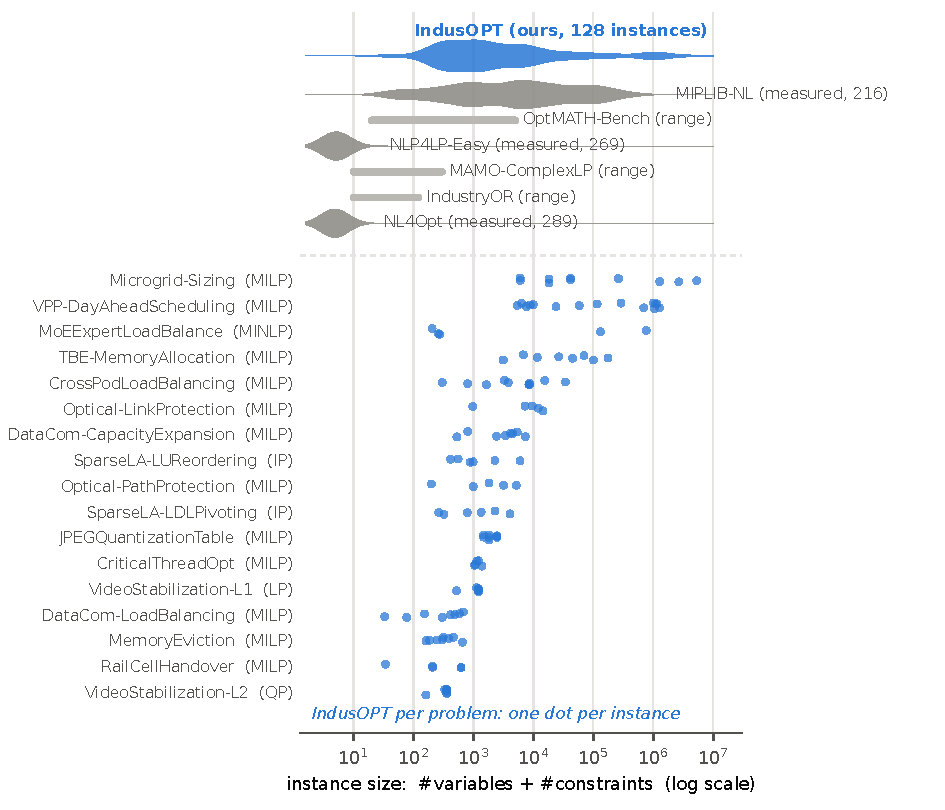
\includegraphics[width=\linewidth]{figs/scale}
\caption{The scale spectrum expressed as \emph{distributions} rather than ranges ($\#\text{vars}+\#\text{cons}$, log scale). Top: silhouette width indicates the density of instances at each size. \bench (blue) reports exact values computed from all \NumInstances{} instances. We additionally report ``measured'' silhouettes computed from public benchmark artifacts (methods and caveats in \texttt{paper/bench\_sizes.json}): all 289 NL4Opt test problems (median size 5, maximum 8), the 269 publicly mirrored NLP4LP easy problems (median 5, maximum 10), and 216 of MIPLIB-NL's 223 instances (median 4{,}879). For MIPLIB-NL, we executed the published ground-truth build scripts against a counting-only solver shim, obtaining digit-exact agreement with MIPLIB~2017 official statistics where comparable. The remaining 7 instances cannot be built from the released artifacts due to a missing shared module, an absent data directory, and one data--code schema mismatch. MAMO, IndustryOR, and OptMATH-Bench release only question text and optimal values; without reference models, per-instance sizes cannot be derived, and therefore only the surveyed ranges~\citep{miplibnl} are shown. Bottom: one dot per \bench instance, per problem.}
\label{fig:scale}
\end{figure}

All statistics reported in this study pertain to a single frozen release, \bench~v1.0, whose manifest and associated commit (\DatasetCommit) are archived with the corpus. Because the repository continues to accept new problem submissions, any description based on “the current repository state” would become outdated by the time of publication. Anchoring the analysis to a fixed manifest ensures that all tables, figures, and the evaluation in Section~\ref{sec:results} reference an identical set of \NumProblems{} problems. Accordingly, problems admitted after the evaluation sweep are not included in v1.0, rather than being reported without corresponding evaluation results.

\bench~v1.0 contains \NumProblems{} problems spanning \NumSubdomains{} sub-domains and \NumInstances{} instances: \NumMILP{} MILP, \NumIP{} IP, \NumLP{} LP, \NumQP{} QP, and \NumMINLP{} MINLP problems (Figure~\ref{fig:scale}). Instance scale is quantified as $\#\text{vars}+\#\text{cons}$ in the reference model, yielding four size bands: \BandSmall{} small ($<10^2$), \BandMedium{} medium ($10^2$--$10^4$), \BandLarge{} large ($10^4$--$10^6$), and \BandVeryLarge{} very large ($\ge 10^6$). The largest instance—microgrid sizing over a multi-year planning horizon—contains \MaxScale{} variables plus constraints; the mixture-of-experts and virtual-power-plant problems likewise exceed $7\times10^5$. Appendix Table~\ref{tab:problems} enumerates all problems together with their model class, instance count, and size range, and Appendix~\ref{app:gallery} summarizes, in one paragraph per problem, the production context, decision variables, and primary sources of difficulty.

\section{Not Every Submission Merits Inclusion of Both a Model and a Solver}
\label{sec:quality}

A benchmark entry comprises five interdependent artifacts that must be mutually consistent. If any one artifact is incorrect, the entry is not merely degraded in quality but becomes actively misleading in one of two ways: it may certify an incorrect model as correct, or it may reject a correct model as incorrect. Either failure mode is more detrimental than omitting the entry entirely, and neither is necessarily self-evident to downstream users. The present section addresses aspects that the aggregate statistics in Section~\ref{sec:dataset} cannot capture: the specific defect classes against which the released corpus was screened, their manifestations in actual submissions, and the corresponding corrective actions. The discussion is intended for users of the benchmark rather than for those seeking to replicate its curation process; accordingly, the purpose of the examples is not to provide a recipe, but to justify the quality claims of the released corpus. A corpus is only as reliable as the set of error modes it is designed to detect. Each screening criterion reported here was induced from at least one submission that violated it, across \NumPullRequests{} reviewed pull requests, of which \NumMergedPRs{} were merged. We identify the affected datasets; the repairs are recorded in the public revision history; and Table~\ref{tab:defects} enumerates all occurrences.

\subsection{Statements that Fail to Uniquely Determine the Model}
\label{sec:q-nl}

The acceptance criterion adopted in practice is a re-derivation test: given access only to the materials available to the model under evaluation—specifically, the problem statement, annotations, data dictionary, and a single sample instance—can an independent modeler reconstruct the reference formulation? If this reconstruction is not possible, the deficiency lies in the statement’s underspecification rather than in the intrinsic difficulty of the task.

The evaluation protocol is stated explicitly because the phrase “we reviewed the statements” does not constitute a reproducible methodology. All \NumProblems{} statements were assessed in a single pass. For each statement, a modeler with access exclusively to the four inputs listed above—and explicitly without access to \texttt{formulation/model.md}, \texttt{code/model.py}, or \texttt{solution/}—constructed a de novo model from the prose description. The optimum of this reconstructed model was then compared with the stored reference objective value under the \ScoreTol{} scoring tolerance. Agreement was interpreted as evidence that the statement uniquely specifies the intended model; disagreement, or an inability to proceed without making unverifiable assumptions, was taken to identify a concrete omission or ambiguity in the prose. The corrective policy was pre-registered and is central to the validity of the procedure: ambiguities were resolved by revising the \emph{statement} rather than altering the model. The directories \texttt{formulation/}, \texttt{code/}, and \texttt{solution/} remained unchanged throughout, ensuring that the reference solutions used for scoring were invariant across this pass and that the before/after comparison reported below is evaluated against a fixed reference. The pass is archived as a single, auditable change set together with per-problem reconstruction outcomes.

Two limitations should be noted. First, reconstruction was conducted with model assistance and subsequently reviewed by the maintainer rather than by an independent cohort; accordingly, the results support the claim that the statements \emph{determine} their associated models, but do not establish that the statements are readily interpretable by domain-naïve readers. Second, the modeler was aware of the existence of a reference solution, although not of its content. Of the \NumProblems{} statements, seven were deemed faithful and were left unchanged, and ten were revised.

\paragraph{Constants available only in the answer key.} In the HarmonyOS thread-scheduling task, the formulation identifies the main thread using a \emph{thread ID} (TID) while aggregating candidate roles using \emph{thread name}. These are opposing identification conventions, and neither was specified in the original statement. Following anonymization, numerous threads share the main thread’s name; consequently, a modeler relying on the statement alone is likely to construct a wake-up forest containing many spurious roots, thereby propagating bias into all downstream statistics. In addition, the tie-breaking constant in the scoring function, $\varepsilon = 10^{-6}$, was provided only in the withheld reference formulation. As a result, participants plausibly substituted alternative values (e.g., $10^{-3}$), yielding systematically inflated objective values. The revised statement (Figure~\ref{fig:ba-statement}) makes both identification conventions and the constant explicit, and performance improved from 0/5 to 5/5 across all four evaluation configurations. This revision operationalizes the principle that \emph{a constant that exists only in the answer key does not constitute legitimate problem difficulty, because it renders the question underdetermined and therefore unanswerable from the public specification.}

\medskip\par\noindent
\baside{\batext{%
\dots The modelling code must reconstruct the wake-up forest from the events:
when \emph{the main thread} issues a wake-up a tree is created \dots
\textbf{After aggregation}, roles whose sample count and critical-hit count
reach the threshold are treated as valid dependencies.\\[3pt]
Each candidate role's benefit \textbf{jointly considers} the critical wake-up
ratio, the critical hit count and the runnable duration. The resource cost is
the \textbf{product} of the priority-gap tier count and the activity tier
count.}}{\batext{%
\dots The \textbf{main thread is one concrete thread instance, not a batch of
same-named threads}: take the TID of the thread in the first wake-up event
named \texttt{main\_comm}, and from then on only that TID is the main thread.
After anonymization several threads share that name, while the rest are
ordinary threads, and this alone determines the shape of the forest. Node
statistics are \textbf{aggregated into roles by thread name}, so that the same
name with a different TID still means one role.\\[3pt]
$s_r=\frac{c_r}{n_r}\cdot c_r\cdot(1+\varepsilon q_r)$, $\varepsilon=10^{-6}$,
with $q_r$ in \textbf{milliseconds}. Both tier counts round \textbf{up} and
count \textbf{at least one tier}.}}
\par\smallskip
\captionof{figure}{A statement that does not determine its model (HarmonyOS thread
scheduling, English gloss of the Chinese original). Left: entity conventions
unstated and the tie-breaking constant $\varepsilon$ present only in the
withheld reference formulation. Right: both conventions and the constant made
explicit. All four evaluation configurations moved from 0/5 to 5/5.}
\label{fig:ba-statement}
\medskip


\paragraph{Multipliers in the objective.} The datacenter load-balancing objective scales each node’s congestion term by an importance multiplier in the range $0.8$--$1.2$, specified in an associated data field. Because this quantity enters exclusively as an objective coefficient (rather than as an explicit constraint), its omission is not detectable via constraint-indexed consistency checks (e.g., no $(C_n)$ identifier exists against which to validate it). After the statement was amended to (i) introduce the weighting explicitly and (ii) describe the intended two-stage aggregation (“peak, then weighted average”), performance of the unannotated configuration increased from 0/8 to 8/8. This has a direct implication for evaluation methodology: prior to the correction, the ablation in Section~\ref{sec:annprobe} would have misattributed the resulting errors to the absence of \emph{annotations}, even though the root cause was a defect in the problem statement.

\paragraph{Two problems, one statement.} The $\ell_1$- and $\ell_2$-based video-stabilization tasks were distributed with byte-identical natural-language statements. The choice of norm is the sole difference between these formulations; it determines the reference solutions and must therefore be specified in the model input. In the absence of any such specification, any solver is necessarily incorrect for at least one of the two tasks. The revision resolves this ambiguity while retaining business-oriented phrasing rather than explicitly naming a norm: one objective prices deviation linearly (“doubling the deviation doubles the cost”), which promotes piecewise-constant velocity segments, whereas the other imposes a superlinear penalty on large deviations, encouraging the optimizer to distribute unavoidable deviation across frames.

\paragraph{The opposite failure: statements that give the modeling away.} The cross-pod load-balancing statement initially encoded key modeling decisions directly in the prose, including the epigraph-style linearization (“traffic may not exceed the product of link capacity and the network-wide maximum utilization”) and the closed-form normalization factor $N(N-1)/2$. These elements effectively pre-specified the mathematical formulation. The revised statement instead confines itself to the operational intent: the operator seeks to minimize worst-direction utilization while using a small number of links; all links have identical unit cost; cost is prorated by the fraction of a link that is provisioned. The formalization is thereby left to the modeler rather than being embedded in the statement.

\subsection{Annotations that mislead}
\label{sec:q-ann}

Curated annotations can be more detrimental than their absence, because they are typically interpreted as authoritative guidance.

In the virtual-power-plant instance, the annotations included a statement that could be construed as permitting omission of the upper-bound component of a positive-part (hinge) formulation. If only the lower envelope $r \ge B_t - P_t$ is imposed, the solver can drive the response variable to any available bound and treat unshaved energy as revenue, thereby yielding an objective value (net cost) that is artificially below the true optimum. The revised text makes explicit that all three inequalities in the standard formulation are required, and clarifies that the original remark is “a corollary of writing it strictly, not a justification for omitting the upper-bound constraints”. Under this correction, the score for the without-annotations configuration increased from 13/15 to 15/15. For the compiler memory-allocation instance, the annotations cited an external address-allocation specification; models followed this reference by introducing address-level decision variables, which spuriously tighten the feasible region and render the batch infeasible. The rewrite explicitly prohibits address-layer variables, improving performance from 0/5 to 5/5.

A third, more subtle failure mode arises when annotations merely restate constraints already present in the problem statement. Reviewers noted that this compromises the discriminative value of the ablation, because identical scores across conditions become uninterpretable: it is unclear whether the base statement was sufficient or whether the annotations contributed no additional information. The revised annotations therefore retain only genuinely out-of-scope restrictions (e.g., no per-image selection, no recomputation of the encoder, and no reformulation as a facility-location problem).

\subsection{Formulations and code that disagree}
\label{sec:q-model}

The compiler memory-allocation submission provides a particularly clear demonstration of why constraint indexing must be verified mechanically. The implementation contained three constraints, $C_{16}$--$C_{18}$, intended to linearize a conjunction over consecutive pipeline-selection decisions, whereas the written formulation terminated at $C_{15}$; moreover, the reference solutions were inherited from a previous version of the model. As a consequence, substitution-based verification failed on all eight instances: the archived solutions referenced nine decision variables that were no longer present in the current model. Consistent with this mismatch, the recorded objective value was 38\% \emph{better} than the true optimum of the model under evaluation (Figure~\ref{fig:ba-code}), because the absence of $C_{18}$ removed the “forcing” inequality and allowed the pipeline-transition variables to remain at zero, thereby avoiding the switching costs they were designed to impose. This example highlights an uncomfortable general failure mode: if the model under test had omitted the same constraints and the answer key remained stale in a compatible way, the two artifacts would have been mutually consistent and automated validation could have accepted an incorrect specification.

\medskip\par\noindent
\baside{\bacode{%
\textbf{formulation/model.md}\\
\dots\\
\#\#\# (C14) Local instantaneous capacity\\
\#\#\# (C15) Kernel outputs end in Global\\[4pt]
\textbf{code/model.py}\\
m.C14 = Constraint(\dots)\\
m.C15 = Constraint(\dots)\\
m.C16 = Constraint(\dots)\\
m.C17 = Constraint(\dots)\\
m.C18 = Constraint(\dots)\\[4pt]
\textbf{checks}\\
check\_model: C16, C17, C18 in code,\\
\phantom{check\_model: }absent from model.md\\
verify\_solution: 0/8\\
inst\_001 key 63.16 vs model 102.38}}{\bacode{%
\textbf{formulation/model.md}\\
\dots\\
\#\#\# (C14) Per-scope instantaneous capacity\\
\#\#\# (C15) All sinks end in Global\\
\#\#\# (C16) $z_{a,b,s}\le h_{a,s-1}$\\
\#\#\# (C17) $z_{a,b,s}\le h_{b,s}$\\
\#\#\# (C18) $z_{a,b,s}\ge h_{a,s-1}+h_{b,s}-1$\\[4pt]
\textbf{code/model.py}\\
m.C14 \dots m.C18 = Constraint(\dots)\\
\phantom{x}\\
\textbf{checks}\\
check\_model: pass\\
\phantom{check\_model: }\\
verify\_solution: 8/8\\
inst\_001 key 102.38 = model 102.38}}
\par\smallskip
\captionof{figure}{Formulation and code disagreeing (compiler memory allocation). The
code carried three constraints linearizing a conjunction of consecutive
pipeline choices, while the formulation stopped at $C_{15}$ and the answer key
came from the previous model generation. The missing $C_{18}$ is the forcing
direction, so the stored objective was 38\% \emph{better} than the model's true
optimum. Had the model under test omitted the same constraints, both sides
would have been self-consistent and every check would have passed.}
\label{fig:ba-code}
\medskip


Implementation defects are typically less subtle but can be equally consequential. In one submission, the \texttt{build()} routine placed a \texttt{max} expression directly in the objective rather than introducing an epigraph formulation, leading the classifier to identify the model as nonlinear and route it to MINLP solvers; both solvers failed to produce a solution. In contrast, the submitter’s private workflow applied a separate linearization, implying that the provided reference solutions corresponded to a different mathematical program than the one processed by the toolchain. In another case, objective weights silently defaulted to hard-coded constants when an optional data file was missing; thus, an instance distributed without that file would be evaluated under weights that were not explicit in the model specification and were not observable to the modeler.

\subsection{Unreliable answer keys}
\label{sec:q-sol}

This category is particularly hazardous because an incorrect reference answer can cause correct models to be rejected without producing an explicit diagnostic, thereby introducing a persistent and hard-to-detect evaluation failure.

\paragraph{A heuristic misrepresented as an answer.} An early sample instance distributed a greedily constructed schedule with objective value 906 as the reference, although the true optimum was 302. Consequently, any model returning 302—the correct solution—would have been scored as incorrect by approximately a factor of three. The explicit \texttt{heuristic} status label prevented this instance from being trusted for adjudication (such instances are excluded from judging rather than treated as ground truth), which motivates the three-valued status convention; the problem was ultimately removed rather than retrofitted.

\paragraph{Claimed optimality without a solver proof.} Four microgrid instances were labeled \texttt{status: optimal} with \texttt{gap: 0.0} (Figure~\ref{fig:ba-key}). However, these solutions were not proven optimal: the solver operated under its default $10^{-4}$ relative MIP gap, and with objective magnitudes around $9.3\times10^6$ this permits absolute deviations of 622--735. This corresponds to relative errors of $6.6$--$7.8\times10^{-5}$, i.e., 66--78 times larger than the $10^{-6}$ scoring tolerance, meaning that correct models could be incorrectly failed. Three aspects make this failure mode noteworthy. First, it was detected not by automated tooling but by an internal inconsistency: one instance’s data strictly contained another’s, yet it reported a \emph{smaller} optimum. Second, substitution-based verification could not detect the issue because the submitted solution is feasible and its reported objective correctly matches that solution. Third, the optimality audit was also misled because it re-solved using the same default tolerance and therefore reproduced the same (non-proven) objective. The audit procedure has since been modified to pin the gap to zero; under this setting it correctly flags four of ten instances as contradicted. Reference solves are now generated with the gap pinned to zero as well.

\medskip\par\noindent
\baside{\bacode{%
\textbf{solution/inst\_003.json}\\
\{ "status": "optimal",\\
\phantom{\{} "objective": 9297616.756461179,\\
\phantom{\{} "bound":\phantom{ctive} 9297616.756461179,\\
\phantom{\{} "gap": 0.0 \}\\[4pt]
\textbf{code/model.py}\\
result = opt.solve(m, \dots)\\
if tc == "optimal":\\
\phantom{xx}status, bound, gap = \\
\phantom{xxxx}"optimal", objective, 0.0\\[4pt]
\textbf{consequence}\\
solver default mip\_rel\_gap = 1e-4\\
true optimum 9296946.42\\
error 670 = 7.2e-5 relative\\
= 72x the 1e-6 scoring tolerance}}{\bacode{%
\textbf{solution/inst\_003.json}\\
\{ "status": "optimal",\\
\phantom{\{} "objective": 9296946.424402560,\\
\phantom{\{} "bound":\phantom{ctive} 9296946.424402560,\\
\phantom{\{} "gap": 0.0 \}\\[4pt]
\textbf{code/model.py}\\
opt.highs\_options = \{\\
\phantom{xx}"mip\_rel\_gap": 0.0,\\
\phantom{xx}"mip\_abs\_gap": 0.0 \}\\
\phantom{x}\\
\textbf{consequence}\\
gap pinned to zero at generation\\
and in the optimality audit\\
audit now reports 4 of 10\\
contradicted, instead of 0}}
\par\smallskip
\captionof{figure}{An answer key that asserts optimality without a corresponding solver certificate (microgrid sizing). A correct model returning 9296946.42 would have been rejected against the recorded 9297616.76. Substitution verification cannot detect this discrepancy because the solution is feasible and its objective matches that solution, and the optimality audit was likewise misled until it also pinned the MIP gap to zero. The issue was identified via a contradiction: one instance’s data was a strict superset of another’s, yet it reported the smaller optimum.}
\label{fig:ba-key}
\medskip


\paragraph{Constructed schedules used as proxies for solver outputs.} The four largest microgrid instances were associated with manually constructed feasible schedules (\texttt{solver: "constructed feasible schedule"}, \texttt{time\_limit\_sec: 0}). For one such instance, a bona fide 600-second optimization run obtained an objective value of $6.55\times10^6$, whereas the recorded reference value was $86.7\times10^6$. Thus, the reference solution was approximately $13\times$ suboptimal; consequently, nearly any reasonable model would appear to outperform the key by roughly an order of magnitude, rendering the comparison non-informative. Re-optimizing these instances using the recorded solutions as warm starts corrected three of the four references. The remaining instance exceeds available memory at $5.3\times10^6$ variables-plus-constraints and therefore continues to retain the constructed schedule; we document this as an open defect rather than omitting the instance.

\paragraph{Reference solution dominated by information contained in the prompt.} For one cross-pod instance, the provided reference objective was 23.7\% worse than a construction explicitly described in the data dictionary, which is supplied to the evaluated model as part of the input. A model that merely implemented this stated construction would therefore generate a solution superior to the answer key yet be scored as incorrect. The issue was addressed by re-solving the instance to align the reference with the described construction. Subsequently, a systematic re-solve further improved seven of the ten references and, for one instance, replaced a degenerate report (\texttt{bound: 0.0, gap: 1.0}) with a meaningful dual bound.

\paragraph{Fabricated optimality bounds.} In one submission, the solution writer populated \texttt{bound} with the incumbent objective and set \texttt{gap} to $0.0$ whenever a valid dual bound was unavailable, thereby converting any feasible solution into an implicit assertion of proven optimality. This constitutes a procedural or instrumentation defect rather than a defect in the underlying instance data; if left uncorrected, it would systematically mislabel future reference solutions generated by the dataset pipeline.

\subsection{Instances that cannot discriminate}
\label{sec:q-inst}

An optimization formulation may be internally consistent yet empirically non-informative when its instance set fails to activate (i.e., render binding) the stated constraints, thereby preventing meaningful discrimination among candidate solutions.

The JPEG quantization-table design task was initially formulated as the selection of a single table from a pre-enumerated candidate set. This representation collapses to a trivial selection problem: under a sole “select exactly one” constraint, the optimum reduces to an $\arg\min$ over the candidate list, and a short exhaustive scan over candidates reproduced all eight reference objective values exactly. Moreover, two of the four constraints further reduced the model’s discriminatory power: the PSNR and FSIM lower bounds were satisfied by every candidate across all instances, so their removal produced no change in the feasible set or in the resulting optimum. In a prior revision of the same benchmark, the intended solution was effectively embedded in the input by providing a data field whose value matched the reference objective to machine precision. Reformulating the task as 64 independent, per-frequency step-size decisions yields a multi-choice knapsack structure with a search space that scales as $\prod_k |C_k|$ and introduces coupling across images through a shared quality requirement. Under this revised structure, the quality constraint becomes decisive: a greedy heuristic now violates it by a factor of 18--28 (Figure~\ref{fig:ba-degenerate}), indicating that the constraint is active and that the instances meaningfully test algorithmic performance.

\medskip\par\noindent
\baside{\bacode{%
\textbf{formulation/model.md}\\
decision: $x_t\in\{0,1\}$ over candidate tables $T$\\
objective: $\min\sum_{i\in I}\sum_{t\in T}S_{t,i}\,x_t$\\
(C1) $\sum_{t\in T}x_t=1$\phantom{xx}exactly one table\\
(C2) PSNR floor per image\\
(C3) FSIM floor per image\\
(C4) $Q_k=\sum_t q_{t,k}x_t$\\[4pt]
\textbf{what it measures}\\
argmin over $|T|$ candidates\\
5-line scan reproduces 8/8 references\\
C2, C3 satisfied by every candidate\\
$\Rightarrow$ deleting them changes nothing}}{\bacode{%
\textbf{formulation/model.md}\\
decision: $x_{k,c}\in\{0,1\}$, step $c$ at frequency $k$\\
objective: $\min\sum_{i}\sum_{k}\sum_{c}R_{i,k,c}\,x_{k,c}$\\
(C1) $\sum_{c\in C_k}x_{k,c}=1\ \forall k$\phantom{x}per frequency\\
(C2) MSE ceiling per image\\
(C3) $Q_k=\sum_c s_{k,c}x_{k,c}$\\
\phantom{x}\\[4pt]
\textbf{what it measures}\\
multi-choice knapsack, $\prod_k|C_k|$\\
greedy violates C2 by 18--28$\times$\\
images coupled through C2\\
$\Rightarrow$ the quality floor now decides}}
\par\smallskip
\captionof{figure}{A formulation whose instance set fails to provide discrimination (JPEG quantization-table design). Left: the original submission reduces to choosing one table from a finite candidate list, i.e., an $\arg\min$ solvable by a brief exhaustive scan, with two of four constraints non-binding on all instances. Right: a reformulation with 64 per-frequency step-size choices coupled by a shared quality ceiling, yielding a substantially larger search space and making the quality constraint decisive.}
\label{fig:ba-degenerate}
\medskip

Analogous degeneration can occur at the instance-data level. In one datacom load-balancing instance, each service provided two path configurations that traversed \emph{identical} link sets. Consequently, all four binary decision combinations induced the same link-utilization profile, and the congestion component of the objective remained constant at $0.503125$. Under these conditions, the model core—comprising link-utilization expressions, per-node time-slot peak constraints, and hard capacity limits—became non-binding, and the purported routing optimization effectively reduced to a trivial binary choice (Figure~\ref{fig:ba-instance}). After regenerating paths such that alternatives used distinct link sets, all three constraint families achieved full 8/8 drop-one coverage.

\medskip\par\noindent
\baside{\bacode{%
\textbf{data/inst\_001/path.csv}\\
id,src,dst,type,weight,\dots,links\\
1,1,5,1,0.4422,\dots,\textbf{1;3;4}\\
2,1,5,2,0.6199,\dots,\textbf{1;3;4}\\
3,2,5,1,0.5250,\dots,\textbf{2;3;4}\\
4,2,5,2,0.8940,\dots,\textbf{2;3;4}\\[4pt]
\textbf{consequence}\\
both options of a service traverse\\
the same links $\Rightarrow$ all four decision\\
combinations give identical utilization,\\
with congestion constant at 0.503125\\
$\Rightarrow$ model body non-binding}}{\bacode{%
\textbf{data/inst\_001/path.csv}\\
id,src,dst,type,weight,\dots,links\\
1,1,6,1,0.6199,\dots,\textbf{1;5;7}\\
2,1,6,2,0.6423,\dots,\textbf{2;6;7}\\
3,2,6,1,0.8940,\dots,\textbf{3;6;7}\\
4,2,6,1,0.8081,\dots,\textbf{3;6;7}\\
5,2,6,2,0.8014,\dots,\textbf{4;5;7}\\[4pt]
\textbf{consequence}\\
options differ in the links they use\\
$\Rightarrow$ the choice moves utilization\\
drop-one coverage C1/C2/C3 = 8/8}}
\par\smallskip
\captionof{figure}{Instance data that lack discriminative power (datacom load balancing). Left: in the submitted instance, the two configurations offered per service traversed identical link sets. Right: after regeneration over distinct link sets, the benchmark decision induces materially different utilizations and therefore changes the objective.}
\label{fig:ba-instance}
\medskip

A submission currently under review exhibits a more subtle manifestation of the same issue. Its objective values (0.27--5) were of comparable magnitude to both the audit cut tolerance ($10^{-6}$) and the solver feasibility tolerance, which in turn led to spurious audit failures. In addition, its residual-threshold constraint was never active in any of 160 pilot runs across eight instances. The appropriate remedy was not to relax tolerances, but to reformulate the objective as an integer-valued count; after this redesign, the audit succeeded without anomalous failures.

\subsection{What the repairs bought, and what they cost}
\label{sec:q-accounting}

\begin{table}[t]
\centering
\small
\caption{Summary of all defect classes observed, including their frequency and the quality-control gate that detected them. Counts reflect distinct defects rather than affected instances (e.g., a single stale answer key that fails eight instances is counted as one defect). The first eight rows are detected by an automated script, whereas the remaining classes require adversarial review, ablation analyses, or detection during evaluation.}
\label{tab:defects}
\begin{tabular}{p{0.24\linewidth}p{0.24\linewidth}r p{0.32\linewidth}}
\toprule
Defect & Caught by & \# & Consequence if shipped \\
\midrule
\DefectRows
\bottomrule
\end{tabular}
\end{table}

Table~\ref{tab:defects} provides a quantitative accounting of the identified issues: \NumDefects{} distinct defects spanning \NumDefectClasses{} defect classes, arising over \NumPullRequests{} pull requests, of which \NumMergedPRs{} were merged. The resulting distribution motivates the adopted toolchain. Specifically, \NumDefectsMechanical{} of \NumDefects{} defects were detected by an automated script executed on every pull request, which justifies the development of such scripts: at this scale, any defect class whose detection depends primarily on manual reviewer attention has a nontrivial probability of reaching release.

However, the partition between mechanically detectable and manually detectable defects is not aligned with an idealized boundary. For example, coverage auditing identifies a defect class that cannot be detected via consistency checks and constitutes the second most productive gate. Conversely, the statement-fidelity defect class—the largest single class (10 defects)—is not detected by any gate. When a problem statement underdetermines the intended model, the formulation, implementation, and solution can remain mutually consistent, causing all automated checks to pass. Detecting such failures required an independent re-derivation pass and, for several problems, surfaced only through the closed-book evaluation results. More generally, corpus quality is constrained by the classes of errors explicitly targeted by the verification process; the mechanical gates operationally define the set of error classes that no longer require manual search.

The accounting should be reported transparently for both conditions. Across the ten revised statements, performance under the with-annotations configuration increased from 55/72 to 71/72. By contrast, the aggregate score for the without-annotations configuration did \emph{not} increase: it remained 55/72, with substantial improvements on three problems offset by regressions on three others. At least one regression appears attributable to a code-generation failure rather than a modeling deficiency, and all results are based on single runs without controlled random seeds. Accordingly, we report the overall aggregate rather than selectively emphasizing the favorable condition. Two additional caveats are warranted. First, completing a statement can legitimately \emph{reduce} the discriminative value of the annotation ablation, because the without-annotations condition may gain information previously unavailable. We accept this trade-off on the grounds that “unanswerable” is distinct from “difficult.” Second, seven of \NumProblems{} statements required no modifications: an audit that identifies no issues in seven cases and identifies issues in ten constitutes a calibrated audit, not an unsuccessful one.

\section{Verification and Evaluation Methodology}
\label{sec:protocol}

Section~\ref{sec:quality} characterized the types of defects that benchmarks of this kind tend to accrue. The present section provides the complementary account: the quality-control gates designed to prevent such defects, the rationale for each gate, the design choices that render the checks sufficiently inexpensive to execute on every pull request, and the empirical yield of these gates on our corpus. We then specify what information is provided to a model under evaluation and what, precisely, is certified by an evaluation verdict.

We document the methodology rather than distribute the toolchain itself. The released corpus includes statements, data, reference formulations, reference implementations, reference solutions, provenance cards, and coverage records; however, the verification and evaluation toolchain is not released (Section~\ref{sec:release}). Consequently, the primary deliverable is the reasoning and specification provided here. For each gate, we therefore present four components sufficient to enable reconstruction or adaptation by the reader: (i) the failure mode it is intended to detect, (ii) the principle by which it operates, (iii) the boundary of what it establishes, and (iv) its observed yield on our corpus.

\subsection{Four gates in the construction chain}
\label{sec:qa}

From an initial business requirement to a certified reference answer, each problem undergoes three successive translations. Each translation is associated with a dedicated quality-control gate, because the corresponding failure modes are distinct (Figure~\ref{fig:pipeline}). A fourth gate evaluates not the intermediate artifacts but the instantiated test cases, namely whether the instances have sufficient discriminatory power to expose a defect.

\begin{figure}[t]
\centering
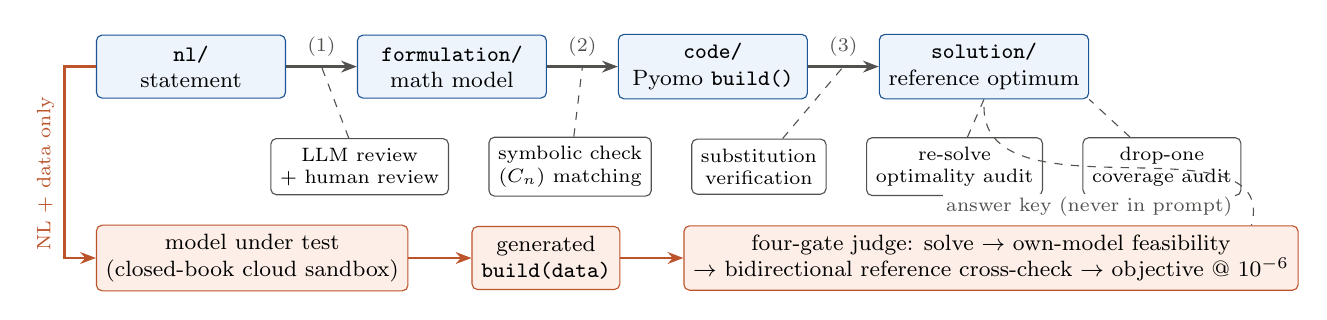
\begin{tikzpicture}[
  font=\footnotesize,
  art/.style={draw=figblue!70!black, fill=figbluebg, rounded corners=2pt,
              minimum height=8mm, minimum width=24mm, align=center},
  gate/.style={draw=figink, fill=white, rounded corners=2pt, align=center,
               minimum height=7mm, font=\scriptsize},
  ev/.style={draw=figorange!80!black, fill=figorangebg, rounded corners=2pt,
             minimum height=8mm, align=center},
  lk/.style={-{Stealth[length=2mm]}, thick, figink},
  glk/.style={figink, dashed, thin},
]
% Construction lane
\node[art] (nl) {\texttt{nl/}\\statement};
\node[art, right=9mm of nl] (form) {\texttt{formulation/}\\math model};
\node[art, right=9mm of form] (code) {\texttt{code/}\\Pyomo \texttt{build()}};
\node[art, right=9mm of code] (sol) {\texttt{solution/}\\reference optimum};
\draw[lk] (nl) -- node[above]{\scriptsize (1)} (form);
\draw[lk] (form) -- node[above]{\scriptsize (2)} (code);
\draw[lk] (code) -- node[above]{\scriptsize (3)} (sol);
% Gates
\node[gate, below=5mm of form.south west, anchor=north west, xshift=-11mm]
  (g1) {LLM review\\$+$ human review};
\node[gate, right=5mm of g1] (g2) {symbolic check\\$(C_n)$ matching};
\node[gate, right=5mm of g2] (g3) {substitution\\verification};
\node[gate, right=5mm of g3] (g4) {re-solve\\optimality audit};
\node[gate, right=5mm of g4] (g5) {drop-one\\coverage audit};
\draw[glk] (g1) -- ($(nl.east)!0.5!(form.west)$);
\draw[glk] (g2) -- ($(form.east)!0.5!(code.west)$);
\draw[glk] (g3) -- ($(code.east)!0.5!(sol.west)$);
\draw[glk] (g4) -- (sol.south);
\draw[glk] (g5) -- (sol.south east);
% Evaluation lane
\node[ev, below=16mm of nl.south west, anchor=north west, minimum width=30mm]
  (llm) {model under test\\(closed-book cloud sandbox)};
\node[ev, right=8mm of llm] (gen) {generated\\\texttt{build(data)}};
\node[ev, right=8mm of gen, minimum width=52mm]
  (judge) {four-gate judge: solve $\to$ own-model feasibility\\
           $\to$ bidirectional reference cross-check $\to$ objective @ $10^{-6}$};
\draw[lk, figorange!80!black] (llm) -- (gen);
\draw[lk, figorange!80!black] (gen) -- (judge);
\draw[lk, figorange!80!black] (nl.west) -- ++(-4mm,0) |- node[pos=0.28, rotate=90, above]
  {\scriptsize NL $+$ data only} (llm.west);
\draw[glk] (sol.south) ++(0,-1mm) to[out=-90,in=75]
  ([xshift=-6mm]judge.north east);
\node[font=\scriptsize, text=figink, anchor=east, fill=white, inner sep=1pt]
  at ($(judge.north east)+(-8mm,2.4mm)$) {answer key (never in prompt)};
\end{tikzpicture}
\caption{The \bench pipeline. Top (blue): the construction chain, in which
each artifact-to-artifact translation is subject to a dedicated gate, and the
answer key is further audited by re-solving and by drop-one-constraint coverage.
Bottom (orange): closed-book evaluation, in which the model under test receives
only the problem statement and data; its generated \texttt{build(data)} is then
executed and scored by the evaluator, while the reference solution is used
exclusively as the answer key.}
\label{fig:pipeline}
\end{figure}

\paragraph{(1) From prose to mathematics: absence of a gate is itself an empirical result.}
A business rule that is omitted prior to formalization remains absent from the subsequent mathematical formulation, implementation, and computed solution; consequently, these artifacts may remain mutually consistent while nevertheless failing to reflect the intended specification. Under such conditions, artifact-level consistency checks cannot detect the omission. This omission category constituted the largest defect class observed (10 of \NumDefects{}, Table~\ref{tab:defects}) and was the only class for which no automated (mechanical) gate was available. The mitigation is therefore procedural: an LLM-based reviewer executes a written checklist for each pull request and iteratively reports issues until no blocking items remain; thereafter, a human maintainer conducts final review and performs the merge, since the automated reviewer does not grant approval and instead only performs the initial routine interrogation. In addition, we apply a periodic re-derivation audit (Section~\ref{sec:q-nl}). Practitioners constructing similar corpora should anticipate that the most prevalent defect mode may be precisely the one not detectable by existing tooling and should allocate resources accordingly.

\paragraph{(2) From mathematics to code: enforce nominal correspondence.}
\emph{Failure mode:} a constraint is present in the mathematical formulation but absent from the code (or conversely), producing a model whose implementation diverges from its documentation and yielding an answer key derived from whichever artifact the submitter executed (Section~\ref{sec:q-model}). \emph{Rationale:} establishing semantic equivalence between \LaTeX{}-encoded constraints and their Pyomo implementation is not practically decidable, and we therefore avoid attempting full equivalence checking. Instead, we impose a naming convention in which each constraint family is numbered $(C_n)$ in the formulation and named \texttt{Cn} in the code. This converts the mapping into a \emph{nominal} correspondence, allowing a simple set comparison to detect missing or extra constraint families within milliseconds, without invoking a solver. The convention introduces negligible overhead for submitters while transforming an intractable verification task into a trivial one. Any intentional omission must be declared via an explicit \texttt{exempt} marker that names the omitted constraint, thereby converting an implicit absence into an explicit, accountable statement. \emph{Scope limitation:} the method establishes only that both artifacts reference the same constraint families; it does not validate that \texttt{C7} in code is semantically identical to $(C_7)$ in the formulation. \emph{Observed impact:} this gate detected the compiler memory-allocation submission in which the code included three constraints absent from the formulation, producing an answer key 38\% better than the model’s true optimum.

\paragraph{(3) From code to solution: substitute rather than solve.}
\emph{Failure mode:} a purported reference solution that is infeasible, or for which the reported objective value is inconsistent with the objective value obtained by evaluating the model at the recorded variable assignment. \emph{Method:} solution verification need not entail re-solving the optimization problem. Instead, reconstruct the model, substitute the recorded assignment, and re-evaluate all constraints and the objective up to \ScoreTol{}. This cleanly separates an inexpensive, deterministic validation task (i.e., feasibility and objective-value consistency) from the computationally intensive task of establishing optimality. The former requires no solver and can therefore be executed in continuous integration for every pull request and every instance, including instances with $5{\times}10^6$ variables that are beyond the capabilities of typical CI runners. \emph{Scope:} this procedure certifies feasibility and correct bookkeeping only; a solution may be feasible and correctly priced yet arbitrarily suboptimal and still pass.

\paragraph{(4) Optimality: reducing an optimality claim to a feasibility test.}
\emph{Failure mode:} a solution labelled \texttt{optimal} that is in fact non-optimal. Such mislabelling can cause correct models to fail silently and persistently, and is particularly hazardous because the dataset may remain internally self-consistent, with disagreement arising only when compared against a stronger solver. \emph{Method:} employ a cut-and-prove strategy. Given a claimed optimum $z^\star$, add a constraint enforcing that the objective strictly improves upon $z^\star$, and re-solve the modified model. If the modified model is infeasible, the optimality claim is validated. This converts an optimality assertion into a feasibility question, which solvers typically address more rapidly and robustly than repeatedly re-deriving an optimum. Two practices are required for methodological soundness. First, solutions explicitly labelled \texttt{heuristic} are exempt and are excluded from judging (Section~\ref{sec:judging}), ensuring that honest non-optimal submissions are not penalized. Second, the optimality gap is fixed to zero, consistent with the lessons described below. \emph{Scope:} certification is performed under a time budget; outcomes are therefore reported as \emph{contradicted}, \emph{consistent}, or \emph{unproven}, where the final category does not constitute evidence of correctness.

\emph{Yield, and a lesson about the auditor auditing itself.} The audit’s procedural history warrants a precise account, because it is straightforward to cite an unduly reassuring summary. When executed on the 13 instances admitted at the time using the solver’s default mixed-integer programming (MIP) optimality gap, the audit produced no contradictions. However, this outcome did not constitute evidence of a fully reliable corpus; rather, it reflected an acceptance tolerance that was too permissive to detect discrepancies. Specifically, an auditor that inherits the default $10^{-4}$ optimality gap will, by construction, certify any deviation permitted by that gap; for objective values on the order of $10^7$, this corresponds to a tolerance that is four orders of magnitude coarser than the scoring tolerance the audit is intended to enforce. After the gap was fixed at zero, the same audit contradicted four of ten microgrid instances (Section~\ref{sec:q-sol}), which were subsequently re-solved and replaced. In its current form—using a zero gap and re-run over the full release underlying this paper—the audit reports \AuditConsistent{} consistent, \AuditUnproven{} unproven, and \AuditContradicted{} contradicted (Appendix~\ref{app:keys}), with \AuditSkipped{} heuristic keys excluded and one disclosed exception tracked as an open defect rather than resolved (the largest microgrid instance; Section~\ref{sec:q-sol}). We present the unproven category explicitly rather than folding it into the consistent count, because doing so would replicate precisely the failure mode induced by the default-gap configuration.

This methodological point has practical consequences rather than merely hypothetical relevance. In an early sample instance, a heuristic schedule with reported cost 906 was distributed as a reference solution, although the true optimum was later proven to be 302; an evaluator that treated the reference label as authoritative would therefore have rejected every correct model. The audit is intended to prevent this class of error from entering the benchmark.

\subsection{Closed-book evaluation}
\label{sec:closedbook}

We evaluate end-to-end performance under a closed-book protocol. Given only the problem statement, the data dictionary, and a single sample instance specifying the required format (optionally supplemented with \texttt{annotations.md}), the model under test is required to generate a Pyomo \texttt{build(data)} function. All generated code is executed by the evaluators on every instance; model-reported metrics are not used.

Each evaluation is executed within an isolated cloud sandbox without repository access. A precondition for accepting any result is verification that the runtime environment corresponds to the intended sandbox, as prior experience revealed a critical failure mode: an SDK fallback silently executed the agent locally with the full repository mounted, thereby exposing the reference formulation, code, and solutions. In that incident, the returned ``generated'' model was verbatim identical to the reference implementation, and no errors were raised. This observation motivates a general requirement: an evaluation that cannot demonstrate environmental isolation is not closed-book, and violations may occur without observable indicators. All results reported in this paper are derived exclusively from runs conducted after this isolation vulnerability was remediated. For reproducibility and auditability, each run archives the exact prompt transmitted to the model, the raw model response, the extracted code, per-instance outputs, and solver logs, enabling any reported figure to be traced to the corresponding generating artifacts.
\subsection{The judging chain}
\label{sec:judging}

A generated model is deemed to have successfully processed an instance only if it passes a four-stage evaluation pipeline:

\begin{enumerate}
\item \textbf{Solvability.} The generated \texttt{build(data)} routine must construct the model and obtain a solution within a sandboxed worker environment, under the pinned solver regime specified below.
\item \textbf{Internal feasibility.} The returned solution is substituted into the \emph{generated} model and all constraints are explicitly re-evaluated. This step is necessary because the solver status alone is not accepted as a sufficient certificate of feasibility.
\item \textbf{Cross-validation against the reference model.} The candidate solution is substituted into the \emph{reference} model, thereby detecting cases in which the generated formulation omits one or more constraints but nevertheless attains an objective value that coincides with the reference optimum. Formally, let $\hat{x}$ denote the generated solution, and let $V$ and $\hat{V}$ denote the variable families of the reference and generated models, respectively. The cross-validation check is defined only when the two namespaces correspond, i.e., when $V=\hat{V}$ up to families that are entirely absent on one side, and yields
  \[
    \mathrm{xval}(\hat{x}) =
    \begin{cases}
      \text{confirmed} & \text{if all reference constraints hold under }\hat{x},\\
      \text{violated}  & \text{if at least one reference constraint is violated},\\
      \text{abstain}   & \text{if a variable family appears on exactly one side.}
    \end{cases}
  \]
  Abstention constitutes an explicit verdict rather than an error condition: eliminating auxiliary variables through substitution is a standard and valid modeling transformation. Consequently, a mismatch in variable spaces more appropriately indicates a non-isomorphic formulation than an incorrect one, and forcing a decision in either direction would introduce avoidable error. Only the \emph{violated} outcome causes an instance to fail.

  The symmetry of this rule is operationally motivated. In the initial deployment, abstention was triggered only when the generated solution introduced variables unknown to the reference model, whereas reference variables absent from the generated solution were implicitly set to zero. Because auxiliary-variable elimination is legitimate, this asymmetric handling incorrectly penalized correct formulations. In one archived sweep, \RejudgeFalseAlarms{} instance-runs produced spurious infeasibility alarms, and \RejudgeFlipped{} verdicts changed when the same archived runs were re-judged off-line without re-executing any model. We report this to emphasize that evaluation procedures require explicit auditing; correctness of a judge should not be presumed in this benchmark or elsewhere.
\item \textbf{Objective agreement.} The objective value must match the reference optimum to within \ScoreTol{} relative or absolute tolerance. Decision-variable assignments are intentionally not compared, since many combinatorial optimization problems admit multiple optimal solutions and direct comparison of $x$ would therefore reject correct models.
\end{enumerate}

Only instances for which the reference solution is certified as \texttt{optimal} are deemed judgeable; in contrast, \texttt{feasible} or \texttt{heuristic} reference solutions render the instance \emph{unjudgeable} rather than implicitly relaxing the answer key (\NumUnjudgeable{} of \NumInstances{} instances in the current release).

\textbf{Solve regime.} Each generated and reference model is evaluated under a single pinned solve regime, which is reported explicitly because pass rates are not interpretable without this context. Solvers are dispatched by model class: LP/MILP instances are routed to HiGHS and then SCIP; QP/NLP instances to Ipopt and then Couenne; and MINLP instances to SCIP and then Couenne. A wall-clock budget of \SolverTimeLimit{}\,s is allocated per solver, and the MIP optimality gap is tightened to $10^{-6}$ to align with the scoring tolerance, since termination at the default $10^{-4}$ gap could lead to incorrect rejection of an otherwise correct model. Both the regime and the dataset contents are version-pinned, and cached results are reused only when both remain unchanged; consequently, modifications to the judge trigger re-evaluation precisely for the affected instance set, avoiding any inadvertent mixture of verdicts produced by different judge versions.

\subsection{Constraint coverage: does the benchmark itself discriminate?}
\label{sec:coverage}

A benchmark instance evaluates a constraint only insofar as the removal of that constraint induces a change in the solution outcome. To operationalize this notion, we quantify \emph{constraint coverage} by deactivating each constraint family in turn, re-solving the instance, and recording the proportion of instances for which the optimal result changes. A constraint family with zero coverage constitutes a methodological blind spot, since a model that systematically omits that family would nonetheless achieve a perfect benchmark score.

Formally, consider a problem with instance set $I$ and constraint families $\{C_n\}$. Let $z(i)$ denote the optimal objective value for instance $i$, and let $z_{\neg n}(i)$ denote the optimal objective value obtained when the constraint family $C_n$ is deactivated. The coverage of $C_n$ is defined as
\[
  \mathrm{cov}(C_n) \;=\; \frac{1}{|I|}\,
  \bigl|\{\, i \in I \;:\; z_{\neg n}(i) \neq z(i)
  \ \text{ or } i \text{ becomes infeasible or unbounded} \,\}\bigr| ,
\]
where objective values are compared using a tolerance of $10^{-9}$. If $\mathrm{cov}(C_n)=0$, then $C_n$ is empirically undetectable under the benchmark distribution: omitting it yields scores identical to those of a correct submission across all available instances. Notably, this metric requires no additional information from \bench beyond an executable reference model and the instance data; consequently, any benchmark that provides reference implementations can compute it directly.

Zero coverage can arise from two distinct mechanisms that require qualitatively different responses. First, the test instances may be insufficiently informative (i.e., too weak), in which case the appropriate remedy is to improve instance design; this occurred in the datacom load-balancing problem, where duplicated path sets rendered three families nonbinding until the paths were regenerated (Section~\ref{sec:q-inst}). Second, a constraint family may be logically implied by the remainder of the model, in which case no instance can induce it to bind and no repair via instance modification is possible. Our single zero-coverage family is of the latter type, a determination that required causal analysis rather than inspection of coverage values alone. In the HarmonyOS thread problem, constraint $C_2$ prohibits boosting a role whose dependency indicator $d_r$ equals zero, while the objective is $\max\sum_r d_r s_r y_r$: such roles contribute exactly zero to the objective yet still consume budget through $C_1$. Consequently, relaxing $C_2$ can only release variables with zero objective value at nonnegative cost, implying that the optimal objective value cannot improve. Empirically, across five instances, 2{,}644 of 3{,}080 roles satisfy $d_r=0$, and the largest associated objective coefficient is $0$. We therefore retain $C_2$ because it formalizes a rule explicitly asserted in the business statement, and we disclose it as a persistent blind spot: any submission omitting $C_2$ attains a perfect score on this family, and will do so for all instances. This distinction is operationally important for metric adopters, because a coverage report that fails to differentiate weak instances from redundant constraints can misdirect effort toward redesigning data in situations where no data revision can alter binding behavior.

Coverage auditing has repeatedly identified genuine blind spots and enables quantification of partial blind spots (e.g., a link-protection exclusivity constraint binding only on the smallest of five instances, and a pivot-block condition binding on one of six). We report problem-level coverage in Section~\ref{sec:results}, provide the full per-family record in Table~\ref{tab:coverage}, and treat weak coverage as an explicit published limitation rather than an internal anomaly: pass rates on a zero-coverage constraint are exactly as informative as the coverage statistic indicates. The audit is not exhaustive, as it spans \NumAudited{} of \NumProblems{} problems; Section~\ref{sec:limitations} details why the metric’s budget is exhausted specifically on the largest instances.

To the best of our knowledge, no existing natural-language-to-optimization benchmark quantifies its discriminative capacity in this manner. Related validation procedures address distinct objectives: MIPLIB-NL verifies that the generated textual description is \emph{sufficient} to reconstruct the underlying model~\citep{miplibnl}, whereas Opti-Agent-Bench evaluates whether a submission is internally consistent across its constituent modules~\citep{optiagentbench}. Both approaches therefore assess self-consistency of an artifact, while coverage evaluates whether the benchmark can reliably distinguish incorrect outputs. These criteria are complementary, and a corpus that includes executable reference models can support all three forms of evaluation.

\subsection{What is released, and what is not}
\label{sec:release}

\bench is released with a narrowly defined objective: to provide researchers and practitioners developing optimization-modeling systems with an industrial-scale corpus against which to evaluate performance and coverage. It is not intended to serve as a general-purpose construction kit. Consequently, the two major components of the project are distributed under different policies.

\textbf{Released: the complete corpus, including keys.} We release the full set of problem statements, annotation files, data dictionaries, and all \NumInstances{} instances, together with a registration card for each problem documenting provenance and the applied desensitization procedure. Critically, we also release the reference formulation, the reference Pyomo implementation, and reference solutions for every instance. In addition, we distribute the per-problem measurements reported in this paper—model class, size statistics, instance axes, and the drop-one coverage record—provided as a \texttt{coverage.json} file in each problem directory, including identified blind spots.

Releasing the keys follows directly from the decision not to distribute the toolchain. A corpus that includes neither reference answers nor an evaluation mechanism is not practically usable as a benchmark; withholding both would also impose dependence on the authors for validation. We acknowledge the associated risks, including the possibility of key contamination and the likelihood that a publicly hosted corpus will eventually be incorporated into pretraining datasets. We address these concerns in Section~\ref{sec:availability} via versioning and controlled updates rather than relying on secrecy.

\textbf{Not released: the toolchain.} Although we describe the toolchain design and rationale, and we report the outcomes of each gate (including identified errors), we do not release the implementation itself. The corpus and the toolchain serve distinct purposes and are governed by substantively different considerations; we therefore separate their release rather than providing a partial release that would inadequately support either objective.

For the \emph{closed-book evaluation harness and the four-gate judge}, the motivation is conventional: when the judging procedure is publicly specified, the benchmark can be systematically optimized against the judge rather than used to measure genuine problem-solving performance. In such settings, the elements most susceptible to strategic overfitting are the scoring logic, prompt templates, and isolation checks; accordingly, these components are retained internally.

This rationale does not extend to the \emph{construction-side quality gates}—consistency, substitution, optimality audit, and coverage—because these checks are executed at problem-admission time rather than at submission-scoring time. Consequently, there is no interactive adversary and little incentive or opportunity for gaming. The actual constraint is more limited and operational: these gates are tightly integrated with this repository’s review records and continuous integration (CI) workflows, some of which depend on internal systems. We are therefore not positioned to support them as a general-purpose, externally maintained package. This is primarily a resourcing decision rather than a security consideration, and the resulting opportunity cost is small. Each gate comprises a modest amount of code operating over artifacts that we already release. Given the published reference models and solutions, for example, the substitution check reduces to a direct traversal of a Pyomo model, while the cut-and-prove audit and the drop-one loop are concise scripts layered over a solver. We have specified all four gates with sufficient precision above to permit independent re-implementation, and we prefer that others implement analogous checks for their own corpora rather than adapt ours. The contribution provided here is thus the design rationale and the empirical evidence that each gate is justified (Table~\ref{tab:defects}), rather than the source code itself.

A consequence of this choice is that our reported results cannot be reproduced by re-running our judge. However, all inputs consumed by the judge and all outputs it produced are externally verifiable: the corpus is public, the archived per-run records are public, and the headline figures reported in this paper are recomputed directly from those archives via \texttt{paper/gen\_numbers.py} rather than manually transcribed. A reader who disputes any reported value can therefore recompute it from the released artifacts. The claim advanced here is falsifiability of the reported results, not end-to-end reproducibility of the full evaluation pipeline.

\subsection{Availability, licensing, versioning, and contamination}
\label{sec:availability}

\textbf{Availability.} \bench~v1.0 corresponds to the tagged release described in Section~\ref{sec:stats} (\DatasetCommit). It is distributed via the project’s public repository and is additionally archived with a DOI, ensuring that citations resolve to an immutable snapshot of the corpus rather than to an evolving branch. The repository serves as the continuously updated development version, whereas the archived release constitutes the fixed artifact evaluated in this study.

\textbf{Licensing.} Problem statements, annotations, data dictionaries, instance data, formulations, and reference solutions are provided for research use under a permissive content licence; reference implementations are released under a permissive software licence. Third-party materials remain subject to their original terms and are not relicensed. Specifically, the SuiteSparse matrices used in the two pivoting problems and the Kodak images underlying the JPEG rate--distortion tables are redistributed under their respective upstream conditions, and each problem’s registration card documents provenance. Two problems are designated with \texttt{internal} sensitivity (Section~\ref{sec:provenance}); their inclusion in the public release is contingent on the same desensitization review applied to the remainder of the suite and is explicitly recorded at the problem level rather than implicitly assumed.

\textbf{Versioning.} Releases are tag-based and immutable. New problems may be introduced between releases; however, a release is issued only in conjunction with re-execution of the full evaluation sweep, thereby preventing mismatches between the corpus composition and the reported results. Reference solutions constitute the sole artifact that may be improved within a release line: if a replay under the pinned regime identifies a strictly better incumbent—initialized from the recorded solution so that outcomes can only match or improve (Appendix~\ref{app:aline})—the corresponding key is updated with an audit trail. In contrast, corpora that permanently freeze such keys at release time accumulate the error mode characterized in Section~\ref{sec:q-sol}.

\textbf{Contamination.} We explicitly acknowledge that public keys are susceptible to contamination and therefore avoid assuming otherwise. To date, the dataset has not been publicly available; consequently, the quantitative results reported in this paper are uncontaminated by construction. However, this property ceases to hold once the corpus is released, and it similarly ceases to hold for any benchmark that discloses its answers. Accordingly, the release incorporates three complementary mitigation measures rather than a single mechanism. First, it includes a canary string, enabling external auditors of future training corpora to directly test whether the dataset has been included. Second, each reported result specifies the release version on which it was obtained, so that a score on v1.0 computed after v1.0 has entered pretraining corpora is not implicitly treated as comparable to results measured prior to public release. Third, subsequent releases will include, for each problem, a private held-out split at the level of instances (as opposed to entire problems), thereby evaluating the same modeling task on data that no submission has previously observed. We emphasize that these measures do not constitute a definitive solution. Rather, the principled position is that a public benchmark can measure uncontaminated capability only once; thereafter, its utility depends primarily on rigorous versioning practices rather than on secrecy.

\textbf{Maintenance.} The repository incorporates new problems via the review pipeline described in Section~\ref{sec:qa}, and identical acceptance criteria apply to submissions originating outside the original development team. Post-release defects are logged and tracked at the level of the affected problem rather than being silently corrected; for example, the open microgrid defect described in Section~\ref{sec:q-sol} is handled under this policy.

\section{Experiments}
\label{sec:results}

\subsection{Setup}

We report the most recent full closed-book sweep involving two commercial code-generation models, \texttt{claude-opus-5} and \texttt{composer-2.5}. Both models were accessed via an identical cloud-agent harness and evaluated under two conditions: with and without \texttt{annotations.md}. The evaluation spans \NumProblems{} problems (\NumRuns{} runs; \NumInstanceRuns{} instance-runs). Among the \NumInstances{} instances, \NumJudgeable{} are judgeable per configuration under the answer-key criterion defined in Section~\ref{sec:judging}. Unless otherwise stated, all results below use the repaired bidirectional cross-check. The archived per-run logs preserve the original verdicts; the subsequent re-judgment is also archived and constitutes a reproducible artifact. Because the harness does not expose sampling temperature or random seed, each table entry corresponds to a single realization rather than an empirical distribution; we discuss the implications in Section~\ref{sec:limitations}.

\subsection{Main results}

\begin{table}[t]
\centering
\small
\caption{Number of passed~/~judgeable instances per problem and configuration (``w/'' = with annotations; ``w/o'' = without). Verdicts are post re-judgment and are recomputed from the archived runs. The primary experimental condition is \emph{without} annotations (Section~\ref{sec:whatapass}). The final three summary rows quantify alternative notions of pass value: (i) the pass rate over the \NumJudgeable{} judgeable instances, which is directly comparable to other benchmarks; (ii) the pass rate over all \NumInstances{} instances, treating the \NumUnjudgeable{} unjudgeable cases as failures, yielding a conservative lower bound; and (iii) the structurally verified rate, which counts only passes whose solutions were actively confirmed within the reference model by the bidirectional cross-check.}
\label{tab:main}
\begin{tabular}{lrr rr rr}
\toprule
& & & \multicolumn{2}{c}{\texttt{composer-2.5}} & \multicolumn{2}{c}{\texttt{claude-opus-5}} \\
\cmidrule(lr){4-5}\cmidrule(lr){6-7}
Problem & Class & Judg. & w/ & w/o & w/ & w/o \\
\midrule
SparseLA-LDLSymmetricPivoting & IP & 6/6 & 6 & 6 & 6 & 6 \\
SparseLA-LUPivotReordering & IP & 6/6 & 6 & 6 & 6 & 6 \\
Camera-JPEGQuantizationTable & MILP & 8/8 & 0 & 8 & 8 & 8 \\
Camera-VideoStabilization-L1 & LP & 8/8 & 8 & 6 & 8 & 8 \\
Camera-VideoStabilization-L2 & QP & 8/8 & 8 & 8 & 8 & 8 \\
Communication-RailCellHandover & MILP & 5/5 & 5 & 5 & 5 & 5 \\
HarmonyOS-CriticalThreadOpt & MILP & 5/5 & 0 & 0 & 0 & 0 \\
HarmonyOS-MemoryEviction & MILP & 8/8 & 8 & 8 & 8 & 8 \\
Cluster-CrossPodLoadBalancing & MILP & 3/10 & 3 & 3 & 3 & 0 \\
TBE-MemoryAllocation & MILP & 5/8 & 5 & 0 & 0 & 4 \\
Microgrid-SizingAndOperation & MILP & 6/10 & 6 & 6 & 0 & 6 \\
VPP-DayAheadLoadScheduling & MILP & 15/15 & 0 & 12 & 15 & 13 \\
DataCom-LoadBalancing & MILP & 8/8 & 8 & 0 & 8 & 0 \\
DataCom-CapacityExpansion & MILP & 8/8 & 8 & 8 & 8 & 8 \\
LLM-MoEExpertLoadBalance & MINLP & 4/5 & 3 & 2 & 3 & 3 \\
OpticalNetwork-LinkProtection & MILP & 5/5 & 5 & 2 & 5 & 5 \\
OpticalNetwork-PathProtection & MILP & 5/5 & 5 & 5 & 5 & 5 \\
\midrule
\textbf{Total passed} & & & \textbf{84} & \textbf{85} & \textbf{96} & \textbf{93} \\
Pass rate (of \NumJudgeable{} judgeable) & & & \ComposerWithAnnPct & \ComposerNoAnnPct & \OpusWithAnnPct & \OpusNoAnnPct \\
Pass rate (of all \NumInstances) & & & \ComposerWithAnnAllPct & \ComposerNoAnnAllPct & \OpusWithAnnAllPct & \OpusNoAnnAllPct \\
\addlinespace[2pt]
\emph{Structurally verified} & & & \StrictComposerWithAnnPct & \StrictComposerNoAnnPct & \StrictOpusWithAnnPct & \StrictOpusNoAnnPct \\
\bottomrule
\end{tabular}
\end{table}

\begin{figure}[t]
\centering
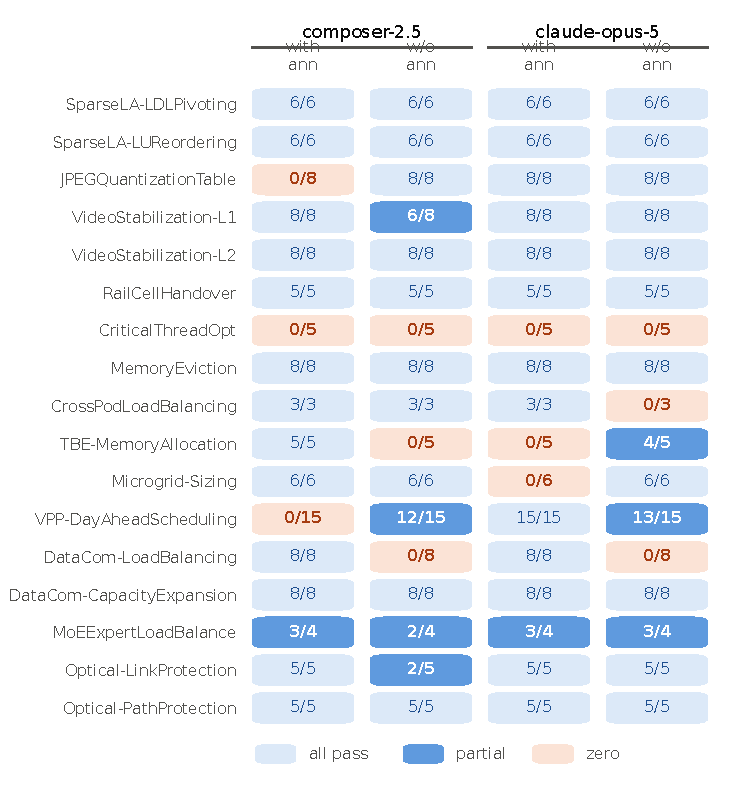
\includegraphics[width=0.72\linewidth]{figs/results_heatmap}
\caption{Compact visualization of Table~\ref{tab:main}: light blue indicates that all judgeable instances pass; dark blue indicates partial success; orange indicates zero passes. Errors are concentrated in a small subset of problems and frequently arise only under particular configurations rather than being uniformly distributed, a pattern more consistent with implicit-constraint satisfaction and world-modeling limitations than with purely stochastic variation.}
\label{fig:heatmap}
\end{figure}

Table~\ref{tab:main} reports the per-problem performance matrix, and Figure~\ref{fig:heatmap} provides a compact visualization of its structure. The stronger model succeeds on \OpusWithAnn{} judgeable instance-runs (\OpusWithAnnPct) when annotations are provided and on \OpusNoAnn{} (\OpusNoAnnPct) without annotations, whereas \texttt{composer-2.5} succeeds on \ComposerWithAnn{} and \ComposerNoAnn{}. We interpret the headline result bidirectionally: embedding a frontier-capability coding model within an effective agent harness now yields solutions for the majority of a forward-constructed industrial corpus, representing a substantive shift relative to the \MiplibBareAvg{} bare-LLM mean (and the at-most-\MiplibSpecialistHi{} specialist results) previously reported for reverse-constructed industrial instances~\citep{miplibnl}. However, this improvement should not be conflated with a claim that \emph{the task is solved}; the benchmark instrumentation is sufficiently granular to characterize precisely how these statements diverge. 

\textbf{The headline metric is computed on the easy-to-verify subset, and we additionally report a conservative bound.} The \NumJudgeable{} judgeable instances exclude \NumUnjudgeable{} instances whose reference solutions could not be certified as optimal by the strongest available open-source solvers; these exclusions are systematic rather than random. All \NumUnjudgeable{} instances arise from four problems (cross-pod balancing, TBE memory allocation, microgrid sizing, MoE placement), which are among the largest-scale cases in the benchmark. Consequently, the judgeable set is biased toward instances that are easier \emph{to verify}, a property that is correlated with being easier to model. When all instances are included and unverifiable cases are conservatively scored as not passed, the same runs yield \OpusWithAnnAllPct{} and \ComposerWithAnnAllPct{}. Both denominators are shown in Table~\ref{tab:main}: the former supports like-for-like comparison, while the latter constitutes an honesty-preserving ceiling under current verification constraints. The commercial-solver replay described in Section~\ref{sec:roadmap} would reclassify some instances from the second denominator into the first; we anticipate that this will reduce, rather than increase, the estimated pass rate.

\textbf{A portion of the measured score derives from information that would not typically be available at deployment time.} The file \texttt{annotations.md} is authored by the engineer responsible for the system and encodes precisely those contextual details that a requirement author may omit. In operational settings, such a document is generally unavailable at the time the requirement is initially transferred and, when recovered, is typically obtained only through iterative clarification. Consequently, the no-annotation condition more closely approximates first contact with an authentic requirement and is therefore treated here as the primary condition. Aggregate score changes can underestimate the effect because they cancel failures that shift in opposing directions: where the ablation is detrimental, it can correspond to the loss of entire problems; conversely, for the virtual-power-plant problem the ablation yields a net improvement of approximately one problem (Section~\ref{sec:annprobe}). The most pronounced case originally reported—datacom load balancing improving from 0/8 without annotations to 8/8 with annotations—was found, upon repeated runs, to be partially attributable to a defect in the task statement rather than an intrinsic effect of the annotations; accordingly, Section~\ref{sec:repeats} retracts this result.

\subsection{What a pass is worth: two tiers, and which one is the headline}
\label{sec:whatapass}

A pass conveys weaker guarantees than may be inferred at face value; however, because \bench retains complete reference solutions, we can quantify this gap precisely. Among the \NumInstanceRuns{} instance-runs, the bidirectional cross-check \emph{explicitly verified} the generated solution within the reference model for \CrossConfirmed{} cases. It abstained for \CrossAbstained{} cases due to non-correspondence between the variable spaces, and it was not executed for the remaining \CrossNotRun{} cases because their references are not certified optimal. The procedure identified \CrossViolated{} genuine violations. Consequently, the majority of passes reported in Table~\ref{tab:main} establish objective agreement (within tolerance) together with feasibility of the solution in the generated model; this evidence remains compatible with a structurally incorrect model that nonetheless attains the correct optimum. Only a small fraction of passes provide evidence of agreement at the level of the reference \emph{model} itself.

Accordingly, we report two pass-rate tiers and state explicitly which inference each tier supports. The \emph{consistent} tier corresponds to the pass rate in Table~\ref{tab:main}: the generated model solves successfully, the returned solution is feasible under that model, and the objective value matches the reference within \ScoreTol{}. This tier is directly comparable to prior work and should be interpreted as a permissive upper bound. The \emph{structurally verified} tier additionally requires that the cross-check confirms (rather than abstains), and it is substantially lower: \StrictOpusNoAnnPct{} for \texttt{claude-opus-5} without annotations, compared with \OpusNoAnnPct{} under the consistent criterion.

The observed gap should not be interpreted as indicating that models fail in 95\% of cases. Rather, it primarily reflects limitations in the evaluator’s coverage rather than model error. The cross-check can be executed only when the generated solution assigns names to variables that also occur in the reference; consequently, it applies mainly to instances whose indexing mirrors the underlying data entities and abstains on valid reformulations that use alternative naming or structure. Accordingly, the set of structurally verified passes is drawn from only \StrictProblems{} out of \NumProblems{} total problems. The principal utility of the strict tier is therefore to bound the inferential claim: for \StrictProblems{} problems, a pass supports the conclusion that the model’s output agrees with the reference, whereas outside this subset no such conclusion can be warranted, irrespective of how many additional passes are observed. Moreover, the strict tier does not saturate, in contrast to the consistent tier, which is close to saturation.

These considerations motivate two reporting choices. First, the primary condition reported throughout is \emph{without} annotations, because it corresponds to the realistic setting in which a requirement is provided for the first time (Section~\ref{sec:annprobe}); the with-annotations condition serves a diagnostic role rather than constituting the primary score. Second, neither tier avoids the partial-oracle problem, as clarified by the coverage audit in Section~\ref{sec:selfmeasure}: one family of constraints is provably undetectable, implying that a model may omit it while still receiving a perfect score under both tiers. The distinguishing feature of \bench is not the absence of this issue—since it arises across benchmarks in this literature—but that it quantifies and reports its own evaluative reach, explicitly indicating where verdicts are unreliable. Benchmarks that do not provide reference models (Section~\ref{sec:related}) cannot perform either audit.

\textbf{Residual errors are highly concentrated, and overall performance exhibits coarse resolution.} Across configurations, both models solve the majority of tasks without error; the remaining failures are dominated by a small subset of problems—specifically, thread scheduling from raw kernel traces, the MINLP expert-placement task, and the two tasks with heuristic reference solutions. The all-zero case (\texttt{CriticalThreadOpt}) fails not due to arithmetic limitations but due to deficient world modeling: in all four configurations, both models infer an empty candidate set from the scheduler traces and consequently collapse to a degenerate single-variable formulation that is reported as “solved,” a failure mode that objective-only scoring on small toy instances would not reveal. This interpretation remains valid, although the all-zero outcome does not: the statement revision in Section~\ref{sec:q-nl} was incorporated after this sweep was archived, and on the current corpus the problem succeeds 5/5 on every repetition (Section~\ref{sec:repeats}). We therefore retain the originally measured row rather than retroactively updating it, because Table~\ref{tab:main} documents a single sweep over a fixed release; silently altering individual cells using a different corpus would undermine auditability of the benchmark.

Because failures cluster at the problem level rather than the instance level, the effective sample size of the sweep is closer to \NumProblems{} than to \NumInstances{}. Moreover, the harness exposes neither temperature nor random seed, implying that small differences between entries in Table~\ref{tab:main} should not be interpreted as a definitive ranking. The per-problem outcome matrix, rather than any aggregate score, constitutes the primary result; uncertainty quantification for aggregates would instead be provided by the repeated-run results referenced in Section~\ref{sec:roadmap}.

Finally, execution time is not the limiting factor; semantic fidelity is. For 13 of 17 problems, solve time is negligible (sub-second to seconds), and the two problems that exhaust the \SolverTimeLimit{}\,s budget are also difficult for the reference pipeline. The discriminative failure modes are incorrect objectives, omitted constraint families, and faulty data binding, consistent with prior observations on reverse-constructed industrial corpora~\citep{miplibnl} and with the failure taxonomy reported in solver-in-the-loop training~\citep{pearl}.

\subsection{Where does the competence live?}
\label{sec:attribution}

The performance reported above should be attributed to an integrated \emph{stack} rather than to an isolated model component. Specifically, the system comprises \texttt{claude-opus-5}; a cloud-based coding agent capable of executing programs, inspecting tracebacks, and iteratively revising outputs; Pyomo together with an open-source solver; a closed-book prompting setup; and, for one experimental condition, an expert-authored annotation file. Each of these layers constitutes a plausible contributor to the observed discrepancy between \OpusWithAnnPct{} in this benchmark and the \MiplibBareAvg{} achieved by nine non-agentic LLMs on reverse-constructed industrial instances of comparable scale, for which five fine-tuned specialist models attain scores at or below \MiplibSpecialistHi{}~\citep{miplibnl}. One layer is already supported by direct empirical evidence: the referenced corpus reports an execution-level failure rate of \MiplibExecFail{}, and its authors argue that these failures largely account for the performance collapse, insofar as many runs terminate before semantic correctness can be evaluated. By design, an agent loop that executes code, reads the traceback, and revises outputs largely eliminates this failure mode; consequently, a substantial portion of the gap is plausibly attributable to the harness rather than to the underlying model. This is presented as a testable hypothesis grounded in existing measurements rather than as a rhetorical concession. Table~\ref{tab:main} is insufficient to disentangle the remaining contributions because both systems reported there are harnessed coding models.

Accordingly, we treat attribution—i.e., the extent to which \OpusWithAnnPct{} derives from the base model versus the agent loop versus the annotation file—as the primary unresolved question that this benchmark is intended to address, rather than as an auxiliary ablation. The design of \bench aims to render this question empirically tractable: the annotation column isolates one layer, while the bare-LLM and agentic rows in Section~\ref{sec:roadmap} isolate the others under an unchanged judging protocol. These measurements are not included in the present paper, and Section~\ref{sec:roadmap} enumerates the obstacles to obtaining each of them. If the harness accounts for most of the observed performance differential, the principal implication for industrial deployment concerns system architecture rather than model selection; however, such a conclusion is only identifiable on a corpus with a sufficiently high performance ceiling to separate layer-wise effects. A benchmark on which all approaches score near zero cannot support meaningful decomposition.

\subsection{The annotation probe}
\label{sec:annprobe}

Because \texttt{annotations.md} explicitly encodes the tacit domain knowledge that an engineer would typically supply when interpreting an otherwise minimal requirement, enabling versus disabling this file provides a controlled perturbation for estimating the extent to which each task’s difficulty is driven by unarticulated constraints. The resulting effects are model-dependent and fall into four categories (Figure~\ref{fig:annprobe}):

\begin{figure}[t]
\centering
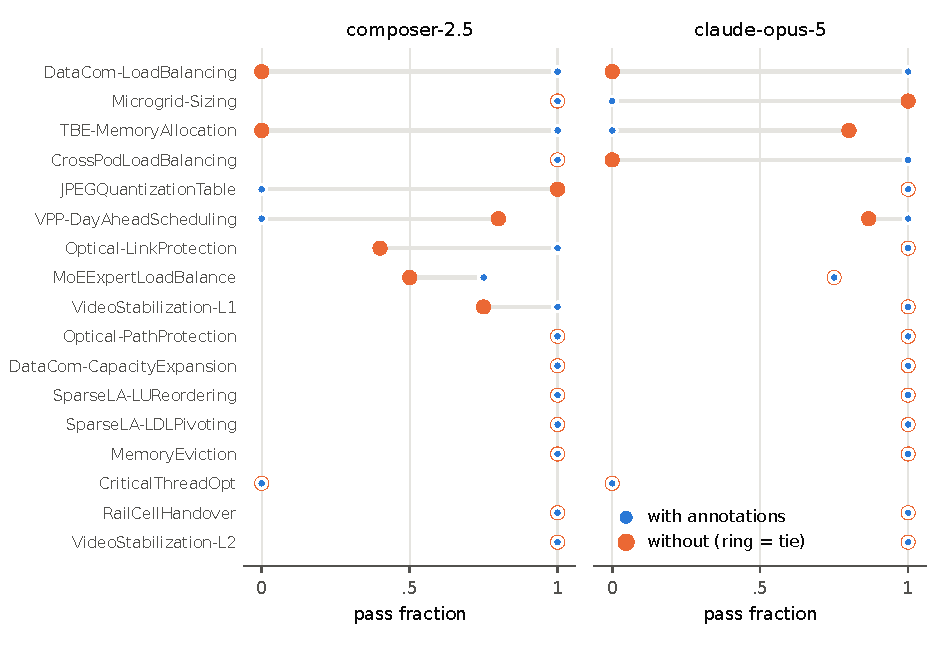
\includegraphics[width=\linewidth]{figs/annotation_probe}
\caption{The annotation probe. For each problem and model, pass fraction with
annotations (blue) vs.\ without (orange), and an orange ring around a blue dot
marks a tie. Problems are ordered by effect size. The probe separates decisive
problems (top) from indifferent ones (bottom), and the same problem can be
decisive for one model and indifferent, or even reversed, for the other.}
\label{fig:annprobe}
\end{figure}

\begin{itemize}
\item \textbf{Decisive, with one retraction.} In the datacom load-balancing task, both models decreased from 8/8 passes with annotations to 0/8 without annotations. We initially interpreted this as strong evidence that a documented implicit constraint (specifically, an epigraph variable capturing peak congestion) constituted essential information for successful solution. However, this finding does not persist under re-execution: after repairing the problem statement, performance in the without-annotations condition becomes unstable rather than uniformly zero, and Section~\ref{sec:repeats} therefore retracts the corresponding claim. The link-protection task remains decisive for one model (5/5 vs.\ 2/5) while being effectively indifferent for the other.
\item \textbf{Reversed.} In the virtual power plant task, one model attains 0/15 \emph{with} annotations but 12/15 without. In this case, the annotation’s informal linearization of demand-response bounds appears to induce an error, whereas the other model incorporates the same text without degradation (15/15). Thus, annotation utility and quality are not invariant across models.
\item \textbf{Indifferent.} Seven tasks exhibit shifts of at most one instance, indicating negligible sensitivity to the presence of annotations.
\item \textbf{Degenerate.} One task yields zero passes in all four conditions, implying that this probe provides no discriminative information for that case.
\end{itemize}

A key methodological implication for benchmark construction is that an ablation gate of this type is effectively necessary to determine whether a given annotation artifact contributes essential information, merely duplicates information already present, or introduces misleading signals; importantly, this determination may be model-dependent.

\subsection{What a zero means: a failure taxonomy}
\label{sec:failures}

When aggregated over the sweep’s failed instance-runs, a recorded score of ``0'' exhibits five distinct failure modes, each with different interpretive consequences:

\begin{enumerate}
\item \textbf{Construction-time crashes}, attributable to Pyomo API misuse
  (\eg defining a variable over an unintended Cartesian product of index sets), such that model instantiation fails and the model object is never created. Three of the four all-zero \emph{cells} in Table~\ref{tab:main} fall into this category and therefore do not reflect modeling inadequacy.
\item \textbf{Degenerate-model fallbacks}, wherein the generated code silently replaces the intended formulation with an empty model when data parsing yields no usable content. Such cases are nevertheless counted as ``executable and solved'', which implies that execution-rate metrics must be interpreted jointly with model-size indicators.
\item \textbf{Overconstrained models}, which are infeasible across all instances; in one case, the generated formulation was approximately an order of magnitude larger than the reference model.
\item \textbf{Solver capitulation}, i.e., syntactically plausible MINLP models for which no available solver attains a solution within the allotted computational budget; these outcomes are recorded as solver failures rather than being attributed to the model specification.
\item \textbf{Judge error}, arising from the corrected cross-check direction described in Section~\ref{sec:judging}; these cases are now zero by construction, but are retained in the taxonomy because benchmarks that do not audit the judging procedure cannot distinguish this failure mode from the preceding categories.
\end{enumerate}

Category (5) warrants emphasis in both respects. Re-judging the archived sweep also quantified the cross-check layer’s \emph{reach}: among \NumInstanceRuns{} instance-runs, it actively confirmed feasibility for \CrossConfirmed{}, abstained for \CrossAbstained{} due to mismatched variable spaces, did not run for \CrossNotRun{} unjudgeable cases, and detected \CrossViolated{} genuine violations in the present sweep. This layer is most effective for problems in which variable indexing corresponds directly to data entities. We state explicitly that, in cases where it abstains, a pass certifies only objective agreement and feasibility of the produced solution, and no stronger guarantee. Constraint coverage (Section~\ref{sec:coverage}) serves as the backstop precisely for these cases.

\subsection{The benchmark measures itself}
\label{sec:selfmeasure}

Two mechanisms render \bench self-correcting in a manner that can be empirically demonstrated rather than merely asserted. First, the drop-one audit now encompasses \NumAudited{} of \NumProblems{} problems and \NumFamiliesAudited{} constraint families (Figure~\ref{fig:coverage}; see Table~\ref{tab:coverage} for the complete per-family record). The audit identifies \NumBlindSpots{} constraint family with zero coverage and an additional \NumWeakFamilies{} families that are binding in fewer than half of their instances. These cases are disclosed as known blind spots, and the redesign of instances to ensure that these constraints become binding is tracked in the repository.

The audit is substantively informative because it can contradict conclusions suggested by aggregate results. Three problems—both sparse-pivoting problems and memory eviction—achieve perfect performance across all four configurations in Table~\ref{tab:main}. However, a perfect score admits two interpretations: either the models are correct, or the problem instances lack discriminative power. Auditing separates these hypotheses, and the outcome is heterogeneous across problems. LU pivot reordering (C2 on 5 of 6) and memory eviction (the weakest family on 4 of 8) remain sound under audit, implying that their perfect scores reflect genuine correctness. In contrast, LDL symmetric pivoting does not: its $C_2$ constraint, the block-strength condition permitting a $2{\times}2$ pivot, alters the optimum in exactly one of six instances. Consequently, a model omitting that condition would still score 6/6 on five instances. This deficiency would not be detectable from pass rates alone, motivating the separate measurement of constraint coverage in addition to overall performance.

\begin{figure}[t]
\centering
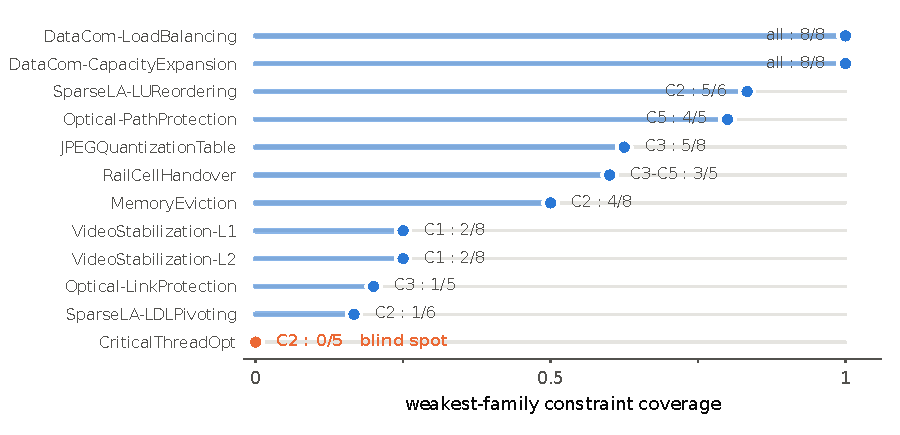
\includegraphics[width=\linewidth]{figs/coverage}
\caption{Constraint coverage of the \NumAudited{} audited problems: for each problem, the \emph{weakest} constraint family and the fraction of instances for which dropping that family changes the optimum. Zero coverage indicates that a model omitting the constraint family achieves a perfect score, which we disclose as a blind spot. The complete per-family record—including the \NumNotAudited{} problems for which drop-one re-solving is computationally prohibitive at their scale—is provided in Table~\ref{tab:coverage}.}
\label{fig:coverage}
\end{figure} Second, the evaluation process directly improved the benchmark: for the cross-pod load-balancing problem, incorporating a generated model’s discrete topology into the \emph{reference} model yielded solutions up to 8.3\% better than those produced by three archived heuristic references. These references were subsequently replaced under the audit trail, with warm-started re-solves used to guarantee non-regression. A benchmark whose answer key can incorporate validated improvements while preserving provenance is expected to remain robust over time relative to one frozen at release.


\subsection{Repeated runs, and what they cost the story}
\label{sec:repeats}

Each entry in Table~\ref{tab:main} corresponds to a single observation. To assess the extent to which this single-sample design affects interpretation, we re-executed the primary condition—\texttt{claude-opus-5} without annotations—\RepeatRuns{} times on the \RepeatProblems{} problems whose instances complete sufficiently quickly to permit repetition. We then evaluate the impact of run-to-run variability on our substantive claims, rather than restricting attention to nominal uncertainty (e.g., error bars).

\textbf{Most entries are stable, but approximately one quarter are not.} For \RepeatStable{} of the \RepeatProblems{} problems, the pass count was identical across all \RepeatRuns{} repetitions. The remaining \RepeatUnstable{} problems exhibited nontrivial variability. This variability is not merely superficial: for example, \texttt{memory eviction} produced pass counts of 8/8, 8/8, and 4/8 across repeats, while \texttt{datacom load balancing} yielded 0/8, 8/8, and 8/8. These cases span the full measurement range for a fixed prompt, a fixed problem, and a fixed model. Consequently, any single execution of a given cell could plausibly yield either maximal success or complete failure, whereas Table~\ref{tab:main} reports exactly one run per cell. The practical implication substantiates a point we previously stated qualitatively: small differences of a few points between cells are not reliably informative under single-run measurement, and per-problem zeros should be re-checked before being interpreted as meaningful failures.

\textbf{Two per-problem narratives in our analysis are not robust to repetition.} These cases merit explicit discussion because they supported key interpretive claims. Table~\ref{tab:main} reports \texttt{CriticalThreadOpt} as zero across all four configurations, and Section~\ref{sec:failures} interprets this as a world-modeling failure. However, on the current corpus the task achieves 5/5 on all three repeats. This discrepancy is attributable not to stochastic run variance but to chronology: the statement revision in Section~\ref{sec:q-nl}, which introduced the entity conventions and the tie-breaking constant, was merged after the sweep used to construct Table~\ref{tab:main} had been archived. Thus, the earlier failure was genuine and its diagnosis was appropriate at the time, but the updated problem formulation no longer manifests the same failure mode.

The second issue is less straightforward. We previously characterized the datacom load-balancing task as the benchmark’s most unambiguous probe of annotation utility, based on an apparent collapse from 8/8 successes with annotations to 0/8 without annotations for both models. Under the revised problem statement, however, the no-annotation condition yields 0/8, 8/8, and 8/8 across repeats. This change is partially attributable to the statement correction: Section~\ref{sec:q-nl} reports the same phenomenon, with performance shifting from 0/8 to 8/8 once the prose explicitly identified the importance weight, and notes that the earlier ablation effectively conflated a statement defect with evidence about annotation dependence. The repeated runs additionally indicate that the remaining effect is unstable rather than cleanly attributable to annotation presence. Accordingly, we retract the strong version of the original claim: on the current corpus, we cannot demonstrate that the annotations for this problem provide necessary information, and one run in three still fails without them for reasons that the single-run design cannot disentangle from stochastic variation. The annotation probe remains methodologically appropriate—indeed, it revealed the underlying defect—but the specific 8/8-to-0/8 result pertains to a corpus version that has since been repaired.

\textbf{Infrastructure is part of the measurement too.} One of the 36 planned runs did not complete: the third link-protection run exhausted its retry budget due to network errors, leaving that cell with two observations rather than three. Of these two runs, one achieved 5/5 and the other 4/5; the latter failed on a single instance due to misuse of the Pyomo API, specifically a constraint rule that returned a bare Boolean. This corresponds to bucket~(1) in the taxonomy above, observed in an in situ run rather than in an archived trace.

\textbf{A language pilot and why it is not yet conclusive.} \bench's statements are in Chinese, which we treat as both a realism feature and an unquantified potential confound. To assess language sensitivity, we translated the \LangPairs{} problems into an English parallel corpus while preserving the original formulations, data, and reference solutions, modifying only the narrative prose. We then executed identical experimental conditions three times per language.

Across the three problems, Chinese and English results were concordant for JPEG (8/8 vs. 8/8) and LU pivot reordering (6/6 vs. 6/6). For memory eviction, the English runs yielded 8/8, 8/8, 8/8, whereas the Chinese runs yielded 8/8, 8/8, 4/8. This discrepancy should not be interpreted as evidence that English is intrinsically easier: the variability observed in Chinese on this task matches the variance reported earlier, and with only three runs per language, stochastic variation is expected to exceed any language effect detectable under this design.

Two additional limitations further constrain interpretation. First, the translation was machine-generated and subsequently reviewed, rather than produced by a native domain expert; thus, any measured performance gap would conflate language comprehension effects with translation fidelity. Second, three problems do not constitute an adequate sample for inference. Accordingly, the pilot supports the usability of the parallel corpus and the feasibility of running the comparison, but it does not provide evidence that language effects are absent.

\subsection{What we have not run, and what it would take}
\label{sec:roadmap}

The preceding study evaluates a single, commonly adopted configuration in the surrounding literature: closed-book frontier code-generation models, assessed with and without annotations. We explicitly delineate untested conditions rather than suggesting comprehensive coverage, because two omissions are directly relevant to the interpretation of Table~\ref{tab:main}.

\textbf{A harness-free control is the most critical missing experiment.} Section~\ref{sec:attribution} posits that the difference between our success rate and the bare-LLM rates on reverse-constructed corpora may be attributable in part to the agentic execution loop rather than the underlying model. Quantifying this effect would require submitting the identical prompts to a standard single-completion interface without any execution or tool use. However, our current evaluation infrastructure is implemented via an agent SDK that does not support such a mode: each invocation is instantiated as an agent with shell access. This is an engineering constraint rather than a substantive claim about causal importance, and it is the reason the attribution in Section~\ref{sec:attribution} is framed as an open question for the benchmark rather than resolved in this work. Notably, the evaluation protocol itself does not preclude this control: any system that produces a Pyomo \texttt{build(data)} artifact is evaluated under the same pinned pipeline.

\textbf{Replaying with a commercial solver would convert a conservative denominator from an upper bound into an empirical quantity.} The \NumUnjudgeable{} unjudgeable instances are unjudgeable because the open-source solvers were unable to certify optimality of their reference solutions (Appendix~\ref{app:keys}); these instances also comprise the largest problems in the corpus. We therefore expect that including them would \emph{decrease} the reported success rate.

Two additional gaps merit explicit mention. First, fine-tuned optimization-specialist models~\citep{orlm,llmopt,sirl} are not evaluated here. A practical impediment is an interface mismatch: these systems typically emit \texttt{coptpy} or \texttt{gurobipy} code for a self-contained prompt, rather than Pyomo code parameterized over a data directory, and inserting a translation layer would introduce confounding. Second, human baselines—reported by ORLM on IndustryOR—would help determine whether the remaining failures reflect instances that are intrinsically challenging for human practitioners as well.

\paragraph{A measured obstacle: the inlining ceiling.}
A substantive impediment to specialist comparison is not attributable to implementation effort. Each released specialist accepts a single, self-contained prompt and provides no auxiliary channel for supplying an external data file; consequently, executing a specialist requires serialising each instance’s data directory into the prompt itself. Empirically quantifying this prompt-budget requirement over \bench yields a median of \InlineMedianKB{}\,KB per instance and a maximum of \InlineMaxMB{}\,MB. Under a conservative assumption of 3.5 bytes per token, \InlineOverSmall{} of \NumInstances{} instances (\InlineOverSmallPct) exceed a 128k-token context window, and \InlineOverLarge{} (\InlineOverLargePct) exceed one million tokens. This constraint should be interpreted as an empirical result rather than an incidental inconvenience: the self-contained prompt interface commonly assumed in the specialist literature exhibits a hard, industrial-scale ceiling that is independent of model quality, and it is not alleviated by fine-tuning.

\section{Limitations}
\label{sec:limitations}

We delineate aspects that the benchmark and the present study do not yet establish, consistent with the paper’s broader emphasis on auditability.

\textbf{Answer-key coverage.} \NumUnjudgeable{} of \NumInstances{} instances have reference solutions whose optimality cannot be established within our audit budget; these instances are therefore excluded from judging. Because these excluded instances are disproportionately difficult, reported pass rates are likely optimistic precisely in the regime that the benchmark is intended to evaluate. Addressing this limitation will require stronger (potentially commercial) solvers and/or larger audit budgets.

\textbf{Instance discriminative power.} Across the \NumAudited{} of \NumProblems{} audited problems, the drop-one metric identifies \NumBlindSpots{} constraint family with zero coverage and \NumWeakFamilies{} families that are binding on fewer than half of their instances. In settings with weak coverage where the cross-check abstains, a passing result certifies only objective agreement and feasibility of the produced solution.

\textbf{Limited scalability of the coverage metric.} The \NumNotAudited{} unaudited problems remain unaudited for a single, structural reason: the drop-one procedure incurs one additional re-solve per family per instance. Consequently, the procedure is economically feasible precisely for small instances and becomes prohibitive precisely for large instances. In the present corpus, a single cross-pod instance requires up to 31 minutes; for the MINLP problem, even a single baseline solve does not terminate reliably; and the largest microgrid instance exhausts available memory. We therefore frame this as a limitation of the proposed metric, rather than solely a limitation of the dataset: the discriminative power of a benchmark is most difficult to certify in the regime where industrial benchmarks most require certification. Lower-cost surrogates—e.g., inspection of dual values or dropping a family only on the smallest instance of each problem—could expand coverage at the expense of rigor; we did not evaluate these alternatives.

\textbf{Single-observation cells.} Because the evaluation harness exposes neither temperature nor random seed, each cell of Table~\ref{tab:main} corresponds to a single run. The repeated-run analysis in Section~\ref{sec:repeats} bounds the associated variability on the tractable half of the corpus: \RepeatUnstable{} of \RepeatProblems{} problems change outcomes between runs, and one problem spans the full observed range. However, this study is limited to a single model under a single experimental condition, and the five largest problems are not repeated at all—precisely the cases where instability would be most consequential and most expensive to quantify. Robust confidence intervals therefore require more repetitions than are available in our experiments.

\textbf{Data origin.} Of the \NumProblems{} problems, \NumOriginSynthetic{} use engineer-authored synthetic data built atop real scenario structure; \NumOriginHybrid{} are hybrid; and \NumOriginReal{} incorporate real measured data. Among the latter, only the HarmonyOS scheduler traces constitute \emph{our} production measurements; the remaining measured datasets are public third-party collections (SuiteSparse, Kodak). Accordingly, our realism claim is grounded primarily in scenario provenance and authorship rather than exclusively in raw measurements. Moreover, desensitization procedures (e.g., rescaling and anonymization) may remove numerical pathologies that occur in production environments.

\textbf{Solver stack.} All auditing and evaluation are performed using open-source solvers (HiGHS, SCIP, Ipopt, Couenne). The MINLP case illustrates that solver capability, rather than modeling expressiveness, can determine what can be adjudicated. Replaying experiments with commercial solvers could strengthen both the answer key and bucket~(4) of the failure taxonomy.

\textbf{Unresolved attribution.} Because both evaluated systems are frontier code-generation models deployed within the same execution-capable agent harness, the present study cannot disentangle the observed pass rate into contributions from (i) base model capability, (ii) the agent-loop implementation, and (iii) the provided annotations; only the third component is isolated in this work. We therefore frame this decomposition as the benchmark’s central unresolved question, rather than as a concluded finding (Section~\ref{sec:attribution}).

\textbf{Ethics, licensing, and data subjects.} The corpus contains no personal data. The only artifact derived from a running production system is an anonymized HarmonyOS \texttt{ftrace} scheduler trace, which logs thread identifiers, wake-up events, and timing information from a device under test (not an end user’s device). Thread and process names are replaced with opaque identifiers, and the identifier mapping is not released. All other measured inputs are sourced from third-party public datasets used under their respective licenses and redistributed without modification, with provenance recorded on a per-problem basis; these include SuiteSparse matrices for the two pivoting tasks and the Kodak image suite underlying the JPEG rate--distortion tables. For scenarios involving commercially sensitive quantities, we apply and explicitly disclose desensitization in the registration card (rather than performing undisclosed transformations): site names are replaced by opaque identifiers, and cost vectors are rescaled by an undisclosed factor selected to preserve the optimizer’s structure. This rescaling is both a safeguard and a substantive limitation, insofar as it may eliminate numerical pathologies that could arise in production deployments. Two problems are labeled \texttt{internal} sensitivity, and their public release follows the same review process as the remaining tasks (Section~\ref{sec:availability}). We consider the most plausible risk to be not information disclosure but the potential misuse or over-interpretation of benchmark scores: passing a problem with weak coverage warrants less confidence than the raw score may suggest. For this reason, the coverage record is distributed with the dataset rather than being documented solely in this manuscript.

\textbf{Scope of the study.} The evaluation is intentionally restricted to two models under a single prompting scheme in a single-shot (closed-book, one-pass) setting. Consequently, the benchmark does not measure multi-turn agentic systems~\citep{optimus,pearl} or fine-tuned specialist models~\citep{orlm,llmopt} on \bench; executing such evaluations constitutes a natural next step. Chinese-language statements are included to improve realism, but they may confound results for models with weaker Chinese comprehension. At present, we do not quantify this effect beyond the \LangPairs{} pilot in Section~\ref{sec:repeats}; in that pilot, the translation is machine-drafted rather than human-authored, and the sample is insufficient to distinguish language effects from the run-to-run variance quantified in the same section.

\section{Conclusion}
\label{sec:conclusion}

\bench conceptualizes industrial natural-language-to-optimization (NL-to-optimization) evaluation as a first-class engineering artifact. Accordingly, the benchmark comprises (i) problem specifications authored prospectively from real production scenarios by the responsible engineers, (ii) instance sets whose scale exceeds that of typical instructional corpora by approximately four orders of magnitude, and (iii) an evaluation judge that is itself version-controlled and audited; notably, the judge was once found to be incorrect and subsequently corrected using archived evidence. Under the strongest configuration, the system succeeds on \OpusWithAnnPct{} of judgeable instance-runs. We release the benchmark not merely because this aggregate score is high, but because it can be systematically decomposed into identifiable contributing factors. Specifically, the score is computed on the subset of instances that are straightforward to verify (\OpusWithAnnAllPct{} when evaluated over all \NumInstances{} instances). A nontrivial fraction of performance is attributable to the availability of an expert annotation file, which is not available at first contact with a requirement and can be decisive (up to an entire problem) when it is required. Moreover, most reported passes reflect objective agreement rather than demonstrated structural equivalence; restricting attention to passes that our cross-check explicitly confirms yields \StrictOpusNoAnnPct{}, and this is measured on a corpus in which one family of constraints is provably undetectable. The per-problem performance matrix, the annotation probe, and the failure taxonomy jointly localize the remaining open problems, including implicit domain constraints, world modeling from raw traces, mixed-integer nonlinear programming (MINLP), and large-scale data binding. In addition, \InlineOverSmall{} instances exceed the point at which the necessary data can be contained within a self-contained prompt. The next question the benchmark is designed to address is how overall performance decomposes among the base model, the surrounding agentic loop, and the domain knowledge provided to the system; a corpus that either saturates or collapses in difficulty cannot support such attribution.


The benchmark’s forward construction is complementary to reverse-engineered corpora such as MIPLIB-NL. Two design principles that we expect to generalize beyond our implementation are: (i) bidirectional cross-validation of a candidate solution against the reference model, and (ii) explicit measurement of whether a given instance is capable of detecting an omitted constraint. These principles are applicable to any benchmark that stores complete solutions rather than scalar answers. We release the corpus to support measurement and comparison by developers of optimization-modeling systems, while retaining the verification and evaluation toolchain (Section~\ref{sec:release}). Consequently, what is published alongside the problem set is the evidentiary substrate—per-problem coverage metrics, audited answer keys, and the blind spots identified in our own data—rather than the evaluation machinery itself. Our central claim is therefore not that the pipeline is fully reproducible, but that the reported results are falsifiable: each reported number is linked to an inspectable problem instance.

\bibliographystyle{plainnat}
\bibliography{refs}

\appendix
\section{Problem Inventory}
\label{app:inventory}

\begin{table}[h]
\centering
\small
\caption{Summary of all \NumProblems{} benchmark problems. ``Size'' is defined as $\#\text{vars}+\#\text{cons}$ in the reference formulation; the reported minimum and maximum are taken over the set of instances for each problem. ``Fam.''\ denotes the number of constraint families that a submission must implement correctly, and ``Int.''\ denotes the proportion of decision variables that are integral; both quantities are computed on the smallest instance of each problem. These structural characteristics capture aspects of formulation complexity that are not determined by size alone, thereby differentiating problems that would otherwise be indistinguishable under a size-based ranking.}
\label{tab:problems}
\begin{tabular}{llrrrrr}
\toprule
Problem & Class & Inst. & Min size & Max size & Fam. & Int. \\
\midrule
\ProblemRows
\bottomrule
\end{tabular}
\end{table}

Size corresponds to the dimension emphasized in Figure~\ref{fig:scale}; however, it is not the sole relevant axis of difficulty, and the two measures do not necessarily covary. The number of constraint families varies from \MinFamilies{} to \MaxFamilies{}, with a median of \MedFamilies{}: for example, the compiler memory-allocation and virtual-power-plant problems require 18 and 17 distinct families, respectively, implying a comparable number of independent opportunities for an incomplete or incorrect specification, whereas the two sparse-pivoting problems attain thousands of variables while involving only two constraint families each. Integrality further partitions the benchmark set rather than inducing a smooth ordering: \NumPureInteger{} of \NumProblems{} problems are purely integral and \NumContinuous{} are purely continuous, with the remainder being genuinely mixed-integer. Consequently, a benchmark characterization based solely on variable counts would place the pivoting problems near the compiler problem despite substantial differences in modelling structure and requirements.

\section{Reference Keys, In Full}
\label{app:keys}

The set of judgeable instances is not determined by any particular submission; instead, it is determined by the strength of the reference key that can be formally established. Table~\ref{tab:keys} reports the reference-solution status for every released instance. Only instances with \texttt{optimal} keys are considered judgeable. Instances labelled \texttt{feasible} or \texttt{heuristic} are excluded from scoring rather than treated as optimal, reflecting the methodological choice to avoid implicitly relying on the weakest available keys (Section~\ref{sec:q-sol}). The \NumUnjudgeable{} excluded instances are concentrated in four problems, all among the largest; as a result, the judgeable denominator is biased toward instances that are comparatively straightforward to verify (Section~\ref{sec:results}).

\begin{table}[h]
\centering
\small
\caption{Reference-solution status by problem. \texttt{optimal} keys are certified under the zero-gap audit; \texttt{feasible} keys include a recorded bound but lack a proof of optimality; and \texttt{heuristic} keys are constructive solutions explicitly labelled as non-certified. Only the first column contributes judgeable instances.}
\label{tab:keys}
\begin{tabular}{lrrrrrc}
\toprule
Problem & Inst. & \texttt{opt.} & \texttt{feas.} & \texttt{heur.} & Judgeable
& Audit \\
\midrule
\KeyRows
\bottomrule
\end{tabular}
\end{table}

The final column reports the outcome of the optimality-audit re-execution for the present release (\texttt{tools/audit\_solution.py}, with the optimality gap fixed to zero), classifying each instance as consistent~/~unproven~/~contradicted. Across all \NumInstances{} instances, the audit yields \AuditConsistent{} consistent, \AuditUnproven{} unproven, and \AuditContradicted{} contradicted outcomes; additionally, \AuditSkipped{} instances are explicitly identified as heuristic and are therefore excluded from the audit. While the absence of contradictions is the desired outcome, it also corresponds to the weaker of two plausible interpretations: \AuditUnproven{} instances remain unresolved because the allotted budget elapsed before the audit could either confirm or refute the certificate. As documented in Section~\ref{sec:q-sol}, there exists a case in which an audit reporting no contradictions was conducted under an overly permissive tolerance, thereby failing to detect existing violations. Consequently, an unproven result should not be construed as evidence of correctness, and we therefore report it as a separate category rather than aggregating it with the consistent cases.

\section{Constraint Coverage, In Full}
\label{app:coverage}

Table~\ref{tab:coverage} reports the full results of the drop-one audit, enumerating, for each audited problem and each constraint family, the number of instances for which deactivating that family yields a different optimal solution. We provide the complete table rather than the weakest-family summary in Figure~\ref{fig:coverage} because the audit toolchain is not included in the release (Section~\ref{sec:release}); consequently, these results constitute the primary evidence available for independent assessment. Families shown in \textbf{bold} exhibit zero coverage, i.e., no instance is sensitive to their removal. The same record is distributed with the corpus as per-problem \texttt{coverage.json} files, enabling benchmark users to interpret their performance on a problem in light of the aspects that the problem instances can (and cannot) empirically discriminate.

\begin{table}[h]
\centering
\small
\caption{Drop-one constraint coverage. Each entry reports $C_n$ followed by the number of instances (out of the total instance count for that problem) for which deactivating $C_n$ changes the optimum. \textbf{Bold} indicates zero coverage (blind spot).}
\label{tab:coverage}
\scriptsize
\begin{tabular}{@{}p{0.33\linewidth}p{0.63\linewidth}@{}}
\toprule
Problem & Coverage per constraint family \\
\midrule
\CoverageRows
\bottomrule
\end{tabular}
\end{table}

\section{Problem Gallery}
\label{app:gallery}

Each problem is described in a single paragraph, specifying (i) the production setting, (ii) the decision variables and objective, and (iii) the primary sources of computational difficulty. The descriptions are maintained at the same level of abstraction as the corresponding published formulations.

\paragraph{CBG-Camera-JPEGQuantizationTable.}
A smartphone imaging pipeline deploys a single $8{\times}8$ JPEG luminance quantization table in firmware, shared across all images rather than optimized on a per-photograph basis. The associated MILP selects, for each of the 64 DCT frequency indices, an integer quantization step size from a finite candidate set so as to minimize the total estimated bitrate over a set of representative images, subject to a strict per-image quality constraint: for every image, the reconstruction PSNR must not fall below its quality-75 baseline, represented after conversion as a constant MSE upper bound~\citep{wallace1992}. Rate and distortion are provided as precomputed per-frequency, per-candidate lookup tables; consequently, the optimization reduces to a purely discrete selection problem under an additive distortion surrogate, and the commonly used per-image table-assignment relaxation is explicitly disallowed. Instances are derived from the public Kodak image suite and vary the number of representative images, the PSNR slack, and the discretization density of the candidate grid.

\paragraph{CBG-Camera-VideoStabilization-L1.}
In handheld video stabilization, a virtual camera trajectory is used to steer a slightly reduced crop window across raw frames to mitigate hand-induced jitter while preserving intentional motion. Each instance corresponds to a single optimization within an online sliding-window procedure: decision variables represent the smoothed 3-DOF camera pose for each currently active frame, and the objective is a weighted $\ell_1$ aggregation of four penalty components (data fidelity, windowed drift, and first- and second-order smoothness). Through the introduction of auxiliary variables, these terms are linearized into an LP whose optimal solutions tend to exhibit piecewise-constant trajectories consistent with cinematic pan behavior, following the $\ell_1$ camera-path stabilization paradigm~\citep{grundmann2011}. Hard constraints enforce that the crop window remains strictly within the image boundaries (via per-frame one-sided corner bounds implied by camera geometry) and ensure continuity with anchor frames fixed from the preceding window. Instances vary in window length (full, tail, cold-start), shake magnitude, crop-margin tightness, and motion regime, while using byte-identical data to the corresponding $\ell_2$ variant.

\paragraph{CBG-Camera-VideoStabilization-L2.}
This benchmark constitutes the quadratic (L2) analogue of the online sliding-window trajectory-smoothing formulation. The four classes of penalty terms are modeled via squared deviations, yielding a convex quadratic program (QP) whose optimal solutions distribute unavoidable corrections across frames. Decision variables remain the per-frame smoothed camera poses, subject to no-black-border cropping constraints and equality constraints that anchor already finalized frames, with a limited lookahead horizon imposed by the device’s finite frame buffer. The instance set is aligned with the corresponding L1 variant, including a square-to-wide aspect-ratio geometry, thereby isolating the impact of the objective norm within an otherwise identical modeling framework.

\paragraph{CBG-Communication-RailCellHandover.}
In high-speed rail and metro deployments, user equipment traverses multiple cells over short time scales; consequently, handover policies driven solely by instantaneous signal measurements can induce ping-pong switching and attachment to dead-end (“island”) cells. To mitigate these effects, a cloud-hosted experience map pre-provisions candidate handover paths to the modem. Given an origin--destination passenger demand distribution, the associated mixed-integer linear program (MILP) selects, for each origin cell, a subset of candidate paths to activate under per-origin budgets on provisioned paths and next-hop options, and assigns each unsplittable flow to an activated path. The objective minimizes passenger-weighted experience costs on nodes and handover edges, augmented with congestion overflow penalties reflecting violations of shared edge-capacity limits. Because paths from distinct origins may merge into common downstream corridors, shared-capacity constraints couple origin-specific subproblems that would otherwise be separable. Instances comprise 6--72 cells and are designed to emphasize distinct operational pathologies, including congestion, island-cell risk, and ping-pong risk.

\paragraph{CBG-HarmonyOS-CriticalThreadOpt.}
During camera cold start, the main thread is coupled to a set of auxiliary threads through scheduler-mediated wakeup chains. Low-priority dependent threads can therefore extend the end-to-end latency along the critical path. To mitigate this effect under a constrained scheduling-intervention budget, the operator selectively raises the priorities of specific thread roles to match the main thread’s priority. The resulting optimization model is a knapsack-style mixed-integer linear program (MILP) defined over thread roles: binary decision variables indicate which roles are boosted; the objective maximizes an aggregate critical-dependency score; and the cost associated with boosting a role is modeled as the product of its priority gap and activity tier. Instance data are derived from real, anonymized \texttt{ftrace} scheduler traces (\texttt{sched\_waking}/\texttt{sched\_switch}). A substantial portion of the complexity is data-driven: constructing the wakeup forest, identifying critical-path membership, estimating role-level statistics, and enforcing eligibility filters requires reconstructing latent structure from raw events via precise rules prior to formulating the optimization problem. This preprocessing stage is also where all four evaluation configurations failed (Section~\ref{sec:failures}).

\paragraph{CBG-HarmonyOS-MemoryEviction.}
A terminal operating system maintains a file-backed page cache at 4\,KB granularity; when the cache is full, eviction decisions directly affect page-fault incidence and thus latency during application launches and UI transitions. Given a recorded access trace and a fixed cache capacity (number of slots), the MILP determines the cache-resident set at each time step and, consequently, the fault events and the identity of each evicted page. The objective minimizes the total number of faults over an offline trace replay, yielding a clairvoyant lower bound in the sense of Belady~\citep{belady1966} that serves as a reference for evaluating online eviction policies. Instances vary in trace length, the ratio between cache capacity and working-set size, and reuse structure (e.g., cyclic working sets, scans with revisits, and interleaved hotspots).

\paragraph{Compute-CAE-SparseLA-LDLSymmetricPivoting.}
For symmetric indefinite linear systems factored in block-diagonal $LDL^{\top}$ form, restricting to $1{\times}1$ diagonal pivots can fail in the presence of near-zero diagonal entries; accordingly, practical algorithms form $2{\times}2$ pivot blocks while maintaining symmetry. This integer program (IP) computes a static pre-ordering in the spirit of Bunch--Kaufman pivoting~\citep{bunchkaufman} by partitioning the index set into $1{\times}1$ and $2{\times}2$ blocks that are simultaneously realizable via a single symmetric permutation. Feasible $1{\times}1$ blocks must satisfy a diagonal-magnitude threshold, whereas feasible $2{\times}2$ blocks must exhibit sufficient block strength. The objective maximizes the product of selected block strengths, yielding a matching-like combinatorial structure with a log-linearized objective. All matrices are real symmetric instances taken verbatim from the public SuiteSparse collection~\citep{suitesparse} (order 48--420), with stability thresholds specified per instance.

\paragraph{Compute-CAE-SparseLA-LUPivotReordering.}
Prior to sparse LU factorization, state-of-the-practice solvers apply row and column permutations to increase the likelihood that numerically dominant entries appear on the diagonal. This IP encodes a static pivot-reordering step as an assignment problem in the classical large-entries-to-the-diagonal formulation~\citep{duffkoster}: select $n$ nonzero entries, with at most one selected per row and per column, to define the permuted diagonal while maximizing the product of selected magnitudes, subject to excluding entries below an instance-specific threshold. Modeling of fill-in effects and any form of dynamic pivoting is intentionally excluded. Instances are derived from unmodified SuiteSparse matrices~\citep{suitesparse} (orders 67--1104), thereby inheriting sparsity structure representative of real engineering applications.

\paragraph{Compute-Cluster-CrossPodLoadBalancing.}
We consider a compute cluster in which pods can be interconnected by identical-capacity, full-duplex links. Directed inter-pod demands must be routed either directly or via exactly one intermediate (transit) pod. The resulting MILP jointly determines (i) which links to install and (ii) how each demand is split across direct and two-hop routes, with the objective of minimizing the maximum directional link utilization plus a pro-rated link construction cost. This provides a compact abstraction of joint topology design and traffic engineering, consistent with models used for reconfigurable datacenter interconnects~\citep{gemini}. The binary topology variables interact nontrivially with the min--max congestion objective, particularly under skewed traffic matrices containing elephant flows. Instances range from 8 to 64 pods; small instances are solved to optimality, whereas industrial-scale instances are reported as \texttt{feasible} together with the best recorded bounds.

\paragraph{Compute-LLM-MoEExpertLoadBalance.}
In Mixture-of-Experts~\citep{moe2017} large language model inference with expert parallelism, concentration of routing mass on a subset of experts can overload individual accelerator cards, thereby increasing end-to-end layer latency. Given forecasts of per-layer, per-expert, per-period load, the optimization assigns experts to cards while exactly filling each card’s available slots; optional redundancy is permitted to replicate high-demand experts. Under non-uniform routing, the model additionally selects traffic-splitting ratios among replicas. The objective minimizes, summed across layers and periods, the maximum (i.e., busiest-card) load. Under uniform routing, the load per replica scales as $1/y$ for $y$ copies, inducing a bilinear dependence that renders the formulation a MINLP; moreover, the expert placement is constrained to remain fixed across all periods. Instances span from instructional cases to near-production configurations (58 layers, 256 experts per layer, 16 cards).

\paragraph{Compute-TBE-MemoryAllocation.}
Following the lowering of fused operators by an operator-fusion compiler into a single kernel’s IR DAG, the runtime must determine a serialized execution order, the execution locus and tiling configuration of each action, and the transfer and placement of intermediate tensors within a memory hierarchy comprising effectively unbounded but high-latency global memory and multiple limited-capacity, low-latency on-chip scopes, each characterized by distinct capacity limits and alignment granularities. The resulting MILP formulation minimizes end-to-end execution time, including computation, data movement costs parameterized by tensor byte volume, and pipeline-switch penalties across DMA, vector, and cube actions. The model enforces precedence constraints, per-scope capacity constraints with explicit alignment and double-buffering overheads, and a terminal condition requiring final outputs to reside in global memory. A trivially feasible schedule that allocates all tensors to global memory always exists; thus, the optimization objective quantifies and exploits the performance benefit of on-chip residency.

\paragraph{Energy-Microgrid-SizingAndOperation.}
An off-grid microgrid supplying a gradually increasing campus demand is co-optimized for capacity expansion and operational dispatch over a 20-year planning horizon. The MILP jointly selects the installed quantities of wind turbines, PV modules, diesel generators, and battery units, allowing batteries to be deployed in discrete staged batches over time, and optimizes dispatch over representative years and intra-year periods. The objective minimizes discounted lifecycle cost, including capital expenditures, operation and maintenance costs, fuel expenditures, and penalty terms for load shedding and renewable curtailment. Key modeling features include exogenous batch-specific battery state-of-health coefficients, PV-specific annual degradation, binary constraints preventing simultaneous charging and discharging, and per-period state-of-charge (SOC) closure conditions. The benchmark set ranges from a 24-period toy instance to the largest instance in the suite (exceeding $5\times10^6$ variables plus constraints), for which heuristic solutions are reported in lieu of proven optimality.

\paragraph{Energy-VPP-DayAheadAdjustableLoadScheduling.}
A virtual power plant (VPP) aggregating multiple distributed sites submits a day-ahead adjustable load profile over 96 fifteen-minute intervals by optimizing each site’s grid purchases, storage charging/discharging decisions, and end-of-period energy states. Site-level constraints enforce nodal power balance with forecast demand and renewable generation, SOC dynamics with asymmetric charging/discharging efficiencies, binary exclusion of simultaneous charging and discharging, and a mandatory return to a specified end-of-day energy target. The objective minimizes procurement cost net of peak-shaving and valley-filling revenues, which are settled at the aggregate VPP level. A crucial implicit constraint is that the service response equals the \emph{positive part} of the deviation between the aggregate purchase schedule and the historical baseline in priced periods; this response is therefore induced by the schedule rather than chosen freely, precluding strategic over-reporting. Instances scale from 4 to 1{,}100 sites, with all instances solved to proven optimality.

\paragraph{ICT-DataCom-LoadBalancing-SingleAndMultitimestamp.}
In a hierarchical enterprise access network, each service at a site is assigned exactly one pre-provisioned path configuration. Within any selected configuration, traffic is split according to fixed weights; consequently, a single discrete configuration choice per service fully determines the induced link-load pattern. The associated MILP minimizes a weighted sum of (i) the importance-weighted peak utilization of site-attached links, (ii) an analogous congestion measure for upper-tier nodes—where each node’s congestion is defined as the maximum utilization over its designated links and over time—and (iii) the fraction of services routed on configurations that violate SLA requirements, subject to hard link-capacity constraints. SLA feasibility is evaluated at the configuration level, such that all constituent paths must simultaneously satisfy delay, jitter, and loss thresholds. This formulation constitutes the benchmark’s most direct annotation probe (Section~\ref{sec:annprobe}). The instance set spans variations in network size, the number of time periods (1--8), the tightness of SLA constraints, and available capacity headroom.

\paragraph{ICT-DataCom-NetworkPlanning-CapacityExpansion.}
A directed backbone/aggregation/edge network supports splittable traffic demands, each of which may be routed over at most four fixed candidate paths. Following a demand shift concentrated in hotspot regions, all incremental demand must be accommodated. The MILP re-optimizes per-service splitting across candidate paths and selects integer-valued capacity expansions via purchasable capacity packs (three discrete sizes exhibiting economies of scale), while enforcing per-link planning-utilization limits of 70--85\% of the post-expansion capacity. The operator’s hierarchical objective—minimize expansion cost first and, conditional on that, minimize traffic migration relative to proportionally scaled baseline splits—is encoded as a single objective using an exact lexicographic weighting provided in the instance data. Each instance is constructed such that a cut surrounding the hotspot region necessitates nontrivial capacity augmentation. Network topologies are synthetic but parameterized to match published PoP-network statistics (11--52 nodes, up to 440 services).

\paragraph{ICT-OpticalNetwork-NetworkPlanning-LinkProtection.}
This problem addresses routing and wavelength assignment (RWA)~\citep{rwareview} in a WDM network with link protection. For each single-link failure scenario—enumerated over all directed links—backup paths and wavelengths are precomputed exclusively for those demands whose working path traverses the failed link. Decision variables include working routes and wavelengths as well as scenario-specific backup routes and wavelengths under a no-wavelength-conversion assumption. Backup provisioning is constrained to avoid any overlap with working link–wavelength resources, and wavelength sharing on a link is disallowed in any network state. The objective minimizes the total number of link–wavelength resources utilized. An additional (implicitly stated) constraint forbids provisioning backup resources for demands unaffected by a given failure. The scenario-wise replication of the constraint system yields large MILPs even for small topologies (e.g., 4--8 nodes), with on the order of $\sim$10,000 constraints.

\paragraph{ICT-OpticalNetwork-NetworkPlanning-PathProtection.}
We consider the companion routing and wavelength assignment (RWA) problem under dedicated (1+1) path protection. Each demand is provisioned with one working path and one link-disjoint backup path, each assigned a single end-to-end wavelength. Backup paths are prohibited from reusing any working link–wavelength resource, and backup capacity is not shared across demands. Moreover, on each link, a given wavelength can be allocated to at most one demand. As in the base formulation, the objective is to minimize the number of occupied link–wavelength pairs, thereby preserving residual capacity (headroom). The resulting “one-backup-per-demand” structure yields substantially more compact mathematical formulations than the corresponding link-protection variant, enabling a controlled comparison of two protection architectures under an identical network-planning task.

\section{Evaluation Inputs and Solve Regime}
\label{app:regime}

This appendix documents (i) the information provided to the model under evaluation and (ii) the procedure by which its output is solved. These two elements are necessary for assessing whether the comparison reported in Section~\ref{sec:results} is methodologically fair. Because the harness that enforces these conditions is not included in the release (Section~\ref{sec:release}), we specify the interface contract rather than the implementation.

\paragraph{Prompt inputs.} Each evaluation call supplies the model with the problem statement, a data dictionary, and the data files for a \emph{single} sampled instance. The instance is truncated to illustrate file structure and formatting while intentionally omitting sufficient information to discourage hard-coding to specific numerical values; the generated code must generalize to all instances of the problem. In the with-annotations configuration, the corresponding annotation file is appended. The reference formulation, reference implementation, and all reference solutions are never provided, and the execution sandbox does not mount the repository. The prompt is written in Chinese, consistent with the problem statements.

\paragraph{Output contract.} The model is required to return a single Python code block that defines \texttt{build(data)}, which constructs and returns a Pyomo \texttt{ConcreteModel} containing the decision variables, exactly one objective function, and all constraints. Four conditions are imposed to ensure that outputs are objectively evaluable. First, \texttt{build} must not invoke a solver, since solving is performed by the caller to ensure a controlled solver configuration. Second, all numerical quantities must be read from \texttt{data}, with no hard-coded constants, so that a single submission can be executed across the full instance set. Third, the argument \texttt{data} is the parsed instance (either a JSON object or a mapping from file stem to file contents, with CSV fields provided as strings). Fourth, only the Python standard library and Pyomo may be used, ensuring reproducibility across evaluation workers.

\paragraph{Solve regime.} The evaluation pipeline applies a model-class-dependent solver rotation: LP/MILP instances are dispatched to HiGHS~\citep{highs} followed by SCIP~\citep{scip}; QP/NLP instances to Ipopt~\citep{ipopt} followed by Couenne~\citep{couenne}; and MINLP instances to SCIP followed by Couenne. Each solver is allocated \SolverTimeLimit{}\,s of wall-clock time, with a MIP relative gap and integrality tolerance set to $10^{-6}$, and a per-worker memory limit enforced. A run terminating with \texttt{optimal} and a bound equal to the reported objective is treated as a proof of optimality. Runs terminating due to the time limit yield an incumbent solution; such incumbents are evaluated using the same objective tolerance and are stored together with the associated bound. The solve regime is version-pinned jointly with the dataset contents; cached results are reused only when both the regime and the dataset remain unchanged. The sweep reported in this paper was generated under a single regime version and subsequently re-evaluated off-line using the corrected cross-check described in Section~\ref{sec:judging}.

\section{Reference-Solution Maintenance}
\label{app:aline}

Reference solutions are maintained as audited, evolving artifacts rather than immutable releases. Each reference model is periodically re-solved under the evaluation regime and warm-started from the previously recorded solution, ensuring that replays can only reproduce or improve upon the stored result and cannot regress. When a strictly better incumbent is obtained, the stored objective value, bound, and optimality gap are updated subject to review. The three improved references described in Section~\ref{sec:selfmeasure} were incorporated into the benchmark through this process, with the corresponding decision log archived. The key design principle is that an answer key capable of incorporating improvements while preserving provenance provides superior long-term stability compared to a release-frozen key, including in cases where improvements are discovered by a system under evaluation.

\end{document}
